\documentclass[11pt]{article} 
\usepackage{acl}


% Standard package includes
\usepackage{times}
\usepackage{latexsym}

\usepackage[T1]{fontenc}

% This assumes your files are encoded as UTF8
\usepackage[utf8]{inputenc}

\usepackage{inconsolata}

\usepackage{microtype}


%additional package(s)
\usepackage{graphicx}
%%%%% NEW MATH DEFINITIONS %%%%%

\usepackage{amsmath,amsfonts,bm}
\usepackage{derivative}
% Mark sections of captions for referring to divisions of figures
\newcommand{\figleft}{{\em (Left)}}
\newcommand{\figcenter}{{\em (Center)}}
\newcommand{\figright}{{\em (Right)}}
\newcommand{\figtop}{{\em (Top)}}
\newcommand{\figbottom}{{\em (Bottom)}}
\newcommand{\captiona}{{\em (a)}}
\newcommand{\captionb}{{\em (b)}}
\newcommand{\captionc}{{\em (c)}}
\newcommand{\captiond}{{\em (d)}}

% Highlight a newly defined term
\newcommand{\newterm}[1]{{\bf #1}}

% Derivative d 
\newcommand{\deriv}{{\mathrm{d}}}

% Figure reference, lower-case.
\def\figref#1{figure~\ref{#1}}
% Figure reference, capital. For start of sentence
\def\Figref#1{Figure~\ref{#1}}
\def\twofigref#1#2{figures \ref{#1} and \ref{#2}}
\def\quadfigref#1#2#3#4{figures \ref{#1}, \ref{#2}, \ref{#3} and \ref{#4}}
% Section reference, lower-case.
\def\secref#1{section~\ref{#1}}
% Section reference, capital.
\def\Secref#1{Section~\ref{#1}}
% Reference to two sections.
\def\twosecrefs#1#2{sections \ref{#1} and \ref{#2}}
% Reference to three sections.
\def\secrefs#1#2#3{sections \ref{#1}, \ref{#2} and \ref{#3}}
% Reference to an equation, lower-case.
\def\eqref#1{equation~\ref{#1}}
% Reference to an equation, upper case
\def\Eqref#1{Equation~\ref{#1}}
% A raw reference to an equation---avoid using if possible
\def\plaineqref#1{\ref{#1}}
% Reference to a chapter, lower-case.
\def\chapref#1{chapter~\ref{#1}}
% Reference to an equation, upper case.
\def\Chapref#1{Chapter~\ref{#1}}
% Reference to a range of chapters
\def\rangechapref#1#2{chapters\ref{#1}--\ref{#2}}
% Reference to an algorithm, lower-case.
\def\algref#1{algorithm~\ref{#1}}
% Reference to an algorithm, upper case.
\def\Algref#1{Algorithm~\ref{#1}}
\def\twoalgref#1#2{algorithms \ref{#1} and \ref{#2}}
\def\Twoalgref#1#2{Algorithms \ref{#1} and \ref{#2}}
% Reference to a part, lower case
\def\partref#1{part~\ref{#1}}
% Reference to a part, upper case
\def\Partref#1{Part~\ref{#1}}
\def\twopartref#1#2{parts \ref{#1} and \ref{#2}}

\def\ceil#1{\lceil #1 \rceil}
\def\floor#1{\lfloor #1 \rfloor}
\def\1{\bm{1}}
\newcommand{\train}{\mathcal{D}}
\newcommand{\valid}{\mathcal{D_{\mathrm{valid}}}}
\newcommand{\test}{\mathcal{D_{\mathrm{test}}}}

\def\eps{{\epsilon}}


% Random variables
\def\reta{{\textnormal{$\eta$}}}
\def\ra{{\textnormal{a}}}
\def\rb{{\textnormal{b}}}
\def\rc{{\textnormal{c}}}
\def\rd{{\textnormal{d}}}
\def\re{{\textnormal{e}}}
\def\rf{{\textnormal{f}}}
\def\rg{{\textnormal{g}}}
\def\rh{{\textnormal{h}}}
\def\ri{{\textnormal{i}}}
\def\rj{{\textnormal{j}}}
\def\rk{{\textnormal{k}}}
\def\rl{{\textnormal{l}}}
% rm is already a command, just don't name any random variables m
\def\rn{{\textnormal{n}}}
\def\ro{{\textnormal{o}}}
\def\rp{{\textnormal{p}}}
\def\rq{{\textnormal{q}}}
\def\rr{{\textnormal{r}}}
\def\rs{{\textnormal{s}}}
\def\rt{{\textnormal{t}}}
\def\ru{{\textnormal{u}}}
\def\rv{{\textnormal{v}}}
\def\rw{{\textnormal{w}}}
\def\rx{{\textnormal{x}}}
\def\ry{{\textnormal{y}}}
\def\rz{{\textnormal{z}}}

% Random vectors
\def\rvepsilon{{\mathbf{\epsilon}}}
\def\rvphi{{\mathbf{\phi}}}
\def\rvtheta{{\mathbf{\theta}}}
\def\rva{{\mathbf{a}}}
\def\rvb{{\mathbf{b}}}
\def\rvc{{\mathbf{c}}}
\def\rvd{{\mathbf{d}}}
\def\rve{{\mathbf{e}}}
\def\rvf{{\mathbf{f}}}
\def\rvg{{\mathbf{g}}}
\def\rvh{{\mathbf{h}}}
\def\rvu{{\mathbf{i}}}
\def\rvj{{\mathbf{j}}}
\def\rvk{{\mathbf{k}}}
\def\rvl{{\mathbf{l}}}
\def\rvm{{\mathbf{m}}}
\def\rvn{{\mathbf{n}}}
\def\rvo{{\mathbf{o}}}
\def\rvp{{\mathbf{p}}}
\def\rvq{{\mathbf{q}}}
\def\rvr{{\mathbf{r}}}
\def\rvs{{\mathbf{s}}}
\def\rvt{{\mathbf{t}}}
\def\rvu{{\mathbf{u}}}
\def\rvv{{\mathbf{v}}}
\def\rvw{{\mathbf{w}}}
\def\rvx{{\mathbf{x}}}
\def\rvy{{\mathbf{y}}}
\def\rvz{{\mathbf{z}}}

% Elements of random vectors
\def\erva{{\textnormal{a}}}
\def\ervb{{\textnormal{b}}}
\def\ervc{{\textnormal{c}}}
\def\ervd{{\textnormal{d}}}
\def\erve{{\textnormal{e}}}
\def\ervf{{\textnormal{f}}}
\def\ervg{{\textnormal{g}}}
\def\ervh{{\textnormal{h}}}
\def\ervi{{\textnormal{i}}}
\def\ervj{{\textnormal{j}}}
\def\ervk{{\textnormal{k}}}
\def\ervl{{\textnormal{l}}}
\def\ervm{{\textnormal{m}}}
\def\ervn{{\textnormal{n}}}
\def\ervo{{\textnormal{o}}}
\def\ervp{{\textnormal{p}}}
\def\ervq{{\textnormal{q}}}
\def\ervr{{\textnormal{r}}}
\def\ervs{{\textnormal{s}}}
\def\ervt{{\textnormal{t}}}
\def\ervu{{\textnormal{u}}}
\def\ervv{{\textnormal{v}}}
\def\ervw{{\textnormal{w}}}
\def\ervx{{\textnormal{x}}}
\def\ervy{{\textnormal{y}}}
\def\ervz{{\textnormal{z}}}

% Random matrices
\def\rmA{{\mathbf{A}}}
\def\rmB{{\mathbf{B}}}
\def\rmC{{\mathbf{C}}}
\def\rmD{{\mathbf{D}}}
\def\rmE{{\mathbf{E}}}
\def\rmF{{\mathbf{F}}}
\def\rmG{{\mathbf{G}}}
\def\rmH{{\mathbf{H}}}
\def\rmI{{\mathbf{I}}}
\def\rmJ{{\mathbf{J}}}
\def\rmK{{\mathbf{K}}}
\def\rmL{{\mathbf{L}}}
\def\rmM{{\mathbf{M}}}
\def\rmN{{\mathbf{N}}}
\def\rmO{{\mathbf{O}}}
\def\rmP{{\mathbf{P}}}
\def\rmQ{{\mathbf{Q}}}
\def\rmR{{\mathbf{R}}}
\def\rmS{{\mathbf{S}}}
\def\rmT{{\mathbf{T}}}
\def\rmU{{\mathbf{U}}}
\def\rmV{{\mathbf{V}}}
\def\rmW{{\mathbf{W}}}
\def\rmX{{\mathbf{X}}}
\def\rmY{{\mathbf{Y}}}
\def\rmZ{{\mathbf{Z}}}

% Elements of random matrices
\def\ermA{{\textnormal{A}}}
\def\ermB{{\textnormal{B}}}
\def\ermC{{\textnormal{C}}}
\def\ermD{{\textnormal{D}}}
\def\ermE{{\textnormal{E}}}
\def\ermF{{\textnormal{F}}}
\def\ermG{{\textnormal{G}}}
\def\ermH{{\textnormal{H}}}
\def\ermI{{\textnormal{I}}}
\def\ermJ{{\textnormal{J}}}
\def\ermK{{\textnormal{K}}}
\def\ermL{{\textnormal{L}}}
\def\ermM{{\textnormal{M}}}
\def\ermN{{\textnormal{N}}}
\def\ermO{{\textnormal{O}}}
\def\ermP{{\textnormal{P}}}
\def\ermQ{{\textnormal{Q}}}
\def\ermR{{\textnormal{R}}}
\def\ermS{{\textnormal{S}}}
\def\ermT{{\textnormal{T}}}
\def\ermU{{\textnormal{U}}}
\def\ermV{{\textnormal{V}}}
\def\ermW{{\textnormal{W}}}
\def\ermX{{\textnormal{X}}}
\def\ermY{{\textnormal{Y}}}
\def\ermZ{{\textnormal{Z}}}

% Vectors
\def\vzero{{\bm{0}}}
\def\vone{{\bm{1}}}
\def\vmu{{\bm{\mu}}}
\def\vtheta{{\bm{\theta}}}
\def\vphi{{\bm{\phi}}}
\def\va{{\bm{a}}}
\def\vb{{\bm{b}}}
\def\vc{{\bm{c}}}
\def\vd{{\bm{d}}}
\def\ve{{\bm{e}}}
\def\vf{{\bm{f}}}
\def\vg{{\bm{g}}}
\def\vh{{\bm{h}}}
\def\vi{{\bm{i}}}
\def\vj{{\bm{j}}}
\def\vk{{\bm{k}}}
\def\vl{{\bm{l}}}
\def\vm{{\bm{m}}}
\def\vn{{\bm{n}}}
\def\vo{{\bm{o}}}
\def\vp{{\bm{p}}}
\def\vq{{\bm{q}}}
\def\vr{{\bm{r}}}
\def\vs{{\bm{s}}}
\def\vt{{\bm{t}}}
\def\vu{{\bm{u}}}
\def\vv{{\bm{v}}}
\def\vw{{\bm{w}}}
\def\vx{{\bm{x}}}
\def\vy{{\bm{y}}}
\def\vz{{\bm{z}}}

% Elements of vectors
\def\evalpha{{\alpha}}
\def\evbeta{{\beta}}
\def\evepsilon{{\epsilon}}
\def\evlambda{{\lambda}}
\def\evomega{{\omega}}
\def\evmu{{\mu}}
\def\evpsi{{\psi}}
\def\evsigma{{\sigma}}
\def\evtheta{{\theta}}
\def\eva{{a}}
\def\evb{{b}}
\def\evc{{c}}
\def\evd{{d}}
\def\eve{{e}}
\def\evf{{f}}
\def\evg{{g}}
\def\evh{{h}}
\def\evi{{i}}
\def\evj{{j}}
\def\evk{{k}}
\def\evl{{l}}
\def\evm{{m}}
\def\evn{{n}}
\def\evo{{o}}
\def\evp{{p}}
\def\evq{{q}}
\def\evr{{r}}
\def\evs{{s}}
\def\evt{{t}}
\def\evu{{u}}
\def\evv{{v}}
\def\evw{{w}}
\def\evx{{x}}
\def\evy{{y}}
\def\evz{{z}}

% Matrix
\def\mA{{\bm{A}}}
\def\mB{{\bm{B}}}
\def\mC{{\bm{C}}}
\def\mD{{\bm{D}}}
\def\mE{{\bm{E}}}
\def\mF{{\bm{F}}}
\def\mG{{\bm{G}}}
\def\mH{{\bm{H}}}
\def\mI{{\bm{I}}}
\def\mJ{{\bm{J}}}
\def\mK{{\bm{K}}}
\def\mL{{\bm{L}}}
\def\mM{{\bm{M}}}
\def\mN{{\bm{N}}}
\def\mO{{\bm{O}}}
\def\mP{{\bm{P}}}
\def\mQ{{\bm{Q}}}
\def\mR{{\bm{R}}}
\def\mS{{\bm{S}}}
\def\mT{{\bm{T}}}
\def\mU{{\bm{U}}}
\def\mV{{\bm{V}}}
\def\mW{{\bm{W}}}
\def\mX{{\bm{X}}}
\def\mY{{\bm{Y}}}
\def\mZ{{\bm{Z}}}
\def\mBeta{{\bm{\beta}}}
\def\mPhi{{\bm{\Phi}}}
\def\mLambda{{\bm{\Lambda}}}
\def\mSigma{{\bm{\Sigma}}}

% Tensor
\DeclareMathAlphabet{\mathsfit}{\encodingdefault}{\sfdefault}{m}{sl}
\SetMathAlphabet{\mathsfit}{bold}{\encodingdefault}{\sfdefault}{bx}{n}
\newcommand{\tens}[1]{\bm{\mathsfit{#1}}}
\def\tA{{\tens{A}}}
\def\tB{{\tens{B}}}
\def\tC{{\tens{C}}}
\def\tD{{\tens{D}}}
\def\tE{{\tens{E}}}
\def\tF{{\tens{F}}}
\def\tG{{\tens{G}}}
\def\tH{{\tens{H}}}
\def\tI{{\tens{I}}}
\def\tJ{{\tens{J}}}
\def\tK{{\tens{K}}}
\def\tL{{\tens{L}}}
\def\tM{{\tens{M}}}
\def\tN{{\tens{N}}}
\def\tO{{\tens{O}}}
\def\tP{{\tens{P}}}
\def\tQ{{\tens{Q}}}
\def\tR{{\tens{R}}}
\def\tS{{\tens{S}}}
\def\tT{{\tens{T}}}
\def\tU{{\tens{U}}}
\def\tV{{\tens{V}}}
\def\tW{{\tens{W}}}
\def\tX{{\tens{X}}}
\def\tY{{\tens{Y}}}
\def\tZ{{\tens{Z}}}


% Graph
\def\gA{{\mathcal{A}}}
\def\gB{{\mathcal{B}}}
\def\gC{{\mathcal{C}}}
\def\gD{{\mathcal{D}}}
\def\gE{{\mathcal{E}}}
\def\gF{{\mathcal{F}}}
\def\gG{{\mathcal{G}}}
\def\gH{{\mathcal{H}}}
\def\gI{{\mathcal{I}}}
\def\gJ{{\mathcal{J}}}
\def\gK{{\mathcal{K}}}
\def\gL{{\mathcal{L}}}
\def\gM{{\mathcal{M}}}
\def\gN{{\mathcal{N}}}
\def\gO{{\mathcal{O}}}
\def\gP{{\mathcal{P}}}
\def\gQ{{\mathcal{Q}}}
\def\gR{{\mathcal{R}}}
\def\gS{{\mathcal{S}}}
\def\gT{{\mathcal{T}}}
\def\gU{{\mathcal{U}}}
\def\gV{{\mathcal{V}}}
\def\gW{{\mathcal{W}}}
\def\gX{{\mathcal{X}}}
\def\gY{{\mathcal{Y}}}
\def\gZ{{\mathcal{Z}}}

% Sets
\def\sA{{\mathbb{A}}}
\def\sB{{\mathbb{B}}}
\def\sC{{\mathbb{C}}}
\def\sD{{\mathbb{D}}}
% Don't use a set called E, because this would be the same as our symbol
% for expectation.
\def\sF{{\mathbb{F}}}
\def\sG{{\mathbb{G}}}
\def\sH{{\mathbb{H}}}
\def\sI{{\mathbb{I}}}
\def\sJ{{\mathbb{J}}}
\def\sK{{\mathbb{K}}}
\def\sL{{\mathbb{L}}}
\def\sM{{\mathbb{M}}}
\def\sN{{\mathbb{N}}}
\def\sO{{\mathbb{O}}}
\def\sP{{\mathbb{P}}}
\def\sQ{{\mathbb{Q}}}
\def\sR{{\mathbb{R}}}
\def\sS{{\mathbb{S}}}
\def\sT{{\mathbb{T}}}
\def\sU{{\mathbb{U}}}
\def\sV{{\mathbb{V}}}
\def\sW{{\mathbb{W}}}
\def\sX{{\mathbb{X}}}
\def\sY{{\mathbb{Y}}}
\def\sZ{{\mathbb{Z}}}

% Entries of a matrix
\def\emLambda{{\Lambda}}
\def\emA{{A}}
\def\emB{{B}}
\def\emC{{C}}
\def\emD{{D}}
\def\emE{{E}}
\def\emF{{F}}
\def\emG{{G}}
\def\emH{{H}}
\def\emI{{I}}
\def\emJ{{J}}
\def\emK{{K}}
\def\emL{{L}}
\def\emM{{M}}
\def\emN{{N}}
\def\emO{{O}}
\def\emP{{P}}
\def\emQ{{Q}}
\def\emR{{R}}
\def\emS{{S}}
\def\emT{{T}}
\def\emU{{U}}
\def\emV{{V}}
\def\emW{{W}}
\def\emX{{X}}
\def\emY{{Y}}
\def\emZ{{Z}}
\def\emSigma{{\Sigma}}

% entries of a tensor
% Same font as tensor, without \bm wrapper
\newcommand{\etens}[1]{\mathsfit{#1}}
\def\etLambda{{\etens{\Lambda}}}
\def\etA{{\etens{A}}}
\def\etB{{\etens{B}}}
\def\etC{{\etens{C}}}
\def\etD{{\etens{D}}}
\def\etE{{\etens{E}}}
\def\etF{{\etens{F}}}
\def\etG{{\etens{G}}}
\def\etH{{\etens{H}}}
\def\etI{{\etens{I}}}
\def\etJ{{\etens{J}}}
\def\etK{{\etens{K}}}
\def\etL{{\etens{L}}}
\def\etM{{\etens{M}}}
\def\etN{{\etens{N}}}
\def\etO{{\etens{O}}}
\def\etP{{\etens{P}}}
\def\etQ{{\etens{Q}}}
\def\etR{{\etens{R}}}
\def\etS{{\etens{S}}}
\def\etT{{\etens{T}}}
\def\etU{{\etens{U}}}
\def\etV{{\etens{V}}}
\def\etW{{\etens{W}}}
\def\etX{{\etens{X}}}
\def\etY{{\etens{Y}}}
\def\etZ{{\etens{Z}}}

% The true underlying data generating distribution
\newcommand{\pdata}{p_{\rm{data}}}
\newcommand{\ptarget}{p_{\rm{target}}}
\newcommand{\pprior}{p_{\rm{prior}}}
\newcommand{\pbase}{p_{\rm{base}}}
\newcommand{\pref}{p_{\rm{ref}}}

% The empirical distribution defined by the training set
\newcommand{\ptrain}{\hat{p}_{\rm{data}}}
\newcommand{\Ptrain}{\hat{P}_{\rm{data}}}
% The model distribution
\newcommand{\pmodel}{p_{\rm{model}}}
\newcommand{\Pmodel}{P_{\rm{model}}}
\newcommand{\ptildemodel}{\tilde{p}_{\rm{model}}}
% Stochastic autoencoder distributions
\newcommand{\pencode}{p_{\rm{encoder}}}
\newcommand{\pdecode}{p_{\rm{decoder}}}
\newcommand{\precons}{p_{\rm{reconstruct}}}

\newcommand{\laplace}{\mathrm{Laplace}} % Laplace distribution

\newcommand{\E}{\mathbb{E}}
\newcommand{\Ls}{\mathcal{L}}
\newcommand{\R}{\mathbb{R}}
\newcommand{\emp}{\tilde{p}}
\newcommand{\lr}{\alpha}
\newcommand{\reg}{\lambda}
\newcommand{\rect}{\mathrm{rectifier}}
\newcommand{\softmax}{\mathrm{softmax}}
\newcommand{\sigmoid}{\sigma}
\newcommand{\softplus}{\zeta}
\newcommand{\KL}{D_{\mathrm{KL}}}
\newcommand{\Var}{\mathrm{Var}}
\newcommand{\standarderror}{\mathrm{SE}}
\newcommand{\Cov}{\mathrm{Cov}}
% Wolfram Mathworld says $L^2$ is for function spaces and $\ell^2$ is for vectors
% But then they seem to use $L^2$ for vectors throughout the site, and so does
% wikipedia.
\newcommand{\normlzero}{L^0}
\newcommand{\normlone}{L^1}
\newcommand{\normltwo}{L^2}
\newcommand{\normlp}{L^p}
\newcommand{\normmax}{L^\infty}

\newcommand{\parents}{Pa} % See usage in notation.tex. Chosen to match Daphne's book.

\DeclareMathOperator*{\argmax}{arg\,max}
\DeclareMathOperator*{\argmin}{arg\,min}

\DeclareMathOperator{\sign}{sign}
\DeclareMathOperator{\Tr}{Tr}
\let\ab\allowbreak

\usepackage{listings}
\usepackage{dsfont}

\definecolor{positional}{HTML}{7777F9}
\definecolor{nonpositional}{HTML}{777777}
\definecolor{lightgray}{HTML}{D3D3D3}

\usepackage{hyperref}
\usepackage{algorithm}
\usepackage{algpseudocode}
\usepackage{url}
\usepackage{graphicx}
\usepackage{booktabs}
\usepackage{colortbl}
\usepackage{enumitem}
\usepackage{linguex}
\usepackage{multirow}

\usepackage[compact]{titlesec}

\setlength{\abovedisplayskip}{2pt}
\setlength{\belowdisplayskip}{2pt}

\newcommand{\yb}[1]{\textcolor{purple}{\small [YB: #1]}}
\newcommand{\tal}[1]{\textcolor{blue}{\small [TAL: #1]}}
\newcommand{\ho}[1]{ \textcolor{ForestGreen}{[HO: #1]}}
\newcommand{\am}[1]{\textcolor{BurntOrange}{[AM: #1]}}

\newcommand{\ob}[2]{$\overbrace{\text{#1}}^{\text{#2}}$}
\newcommand{\ub}[2]{$\underbrace{\text{#1}}_{\text{#2}}$}


\title{Position-aware Automatic Circuit Discovery}

\author{
Tal Haklay$^1$  \quad Hadas Orgad$^1$  \quad David Bau$^2$  \quad Aaron Mueller$^{1,2}$  \quad Yonatan Belinkov$^1$  \\
$^1$Technion -- Israel Institute of Technology \quad $^2$Northeastern University \\[1ex]
\{\href{mailto:tal.ha@campus.ac.il}{\texttt{tal.ha}},
\href{mailto:orgad.hadas@campus.technion.ac.il}{\texttt{orgad.hadas}}\}\texttt{@campus.ac.il},
\{\href{mailto:d.bau@northeastern.edu}{\texttt{d.bau}},
\href{mailto:aa.mueller@northeastern.edu}{\texttt{aa.mueller}}\}\texttt{@northeastern.edu} \\
\href{mailto:belinkov@technion.ac.il}{\texttt{belinkov@technion.ac.il}}
}


\newcommand{\fix}{\marginpar{FIX}}
\newcommand{\new}{\marginpar{NEW}}

% formalisms:
% metric = m
% model = \mathcal{M}; circuit = \mathcal{C}
% empty model = \varnothing
% faithfulness = F
% token position = t; token span = T
% task = \mathcal{T}


\begin{document}


\maketitle

\begin{abstract}
  In this work, we present a novel technique for GPU-accelerated Boolean satisfiability (SAT) sampling. Unlike conventional sampling algorithms that directly operate on conjunctive normal form (CNF), our method transforms the logical constraints of SAT problems by factoring their CNF representations into simplified multi-level, multi-output Boolean functions. It then leverages gradient-based optimization to guide the search for a diverse set of valid solutions. Our method operates directly on the circuit structure of refactored SAT instances, reinterpreting the SAT problem as a supervised multi-output regression task. This differentiable technique enables independent bit-wise operations on each tensor element, allowing parallel execution of learning processes. As a result, we achieve GPU-accelerated sampling with significant runtime improvements ranging from $33.6\times$ to $523.6\times$ over state-of-the-art heuristic samplers. We demonstrate the superior performance of our sampling method through an extensive evaluation on $60$ instances from a public domain benchmark suite utilized in previous studies. 


  
  % Generating a wide range of diverse solutions to logical constraints is crucial in software and hardware testing, verification, and synthesis. These solutions can serve as inputs to test specific functionalities of a software program or as random stimuli in hardware modules. In software verification, techniques like fuzz testing and symbolic execution use this approach to identify bugs and vulnerabilities. In hardware verification, stimulus generation is particularly vital, forming the basis of constrained-random verification. While generating multiple solutions improves coverage and increases the chances of finding bugs, high-throughput sampling remains challenging, especially with complex constraints and refined coverage criteria. In this work, we present a novel technique that enables GPU-accelerated sampling, resulting in high-throughput generation of satisfying solutions to Boolean satisfiability (SAT) problems. Unlike conventional sampling algorithms that directly operate on conjunctive normal form (CNF), our method refines the logical constraints of SAT problems by transforming their CNF into simplified multi-level Boolean expressions. It then leverages gradient-based optimization to guide the search for a diverse set of valid solutions.
  % Our method specifically takes advantage of the circuit structure of refined SAT instances by using GD to learn valid solutions, reinterpreting the SAT problem as a supervised multi-output regression task. This differentiable technique enables independent bit-wise operations on each tensor element, allowing parallel execution of learning processes. As a result, we achieve GPU-accelerated sampling with significant runtime improvements ranging from $10\times$ to $1000\times$ over state-of-the-art heuristic samplers. Specifically, we demonstrate the superior performance of our sampling method through an extensive evaluation on $60$ instances from a public domain benchmark suite utilized in previous studies.

\end{abstract}

\begin{IEEEkeywords}
Boolean Satisfiability, Gradient Descent, Multi-level Circuits, Verification, and Testing.
\end{IEEEkeywords}
\section{Introduction}
\label{section:introduction}

% redirection is unique and important in VR
Virtual Reality (VR) systems enable users to embody virtual avatars by mirroring their physical movements and aligning their perspective with virtual avatars' in real time. 
As the head-mounted displays (HMDs) block direct visual access to the physical world, users primarily rely on visual feedback from the virtual environment and integrate it with proprioceptive cues to control the avatar’s movements and interact within the VR space.
Since human perception is heavily influenced by visual input~\cite{gibson1933adaptation}, 
VR systems have the unique capability to control users' perception of the virtual environment and avatars by manipulating the visual information presented to them.
Leveraging this, various redirection techniques have been proposed to enable novel VR interactions, 
such as redirecting users' walking paths~\cite{razzaque2005redirected, suma2012impossible, steinicke2009estimation},
modifying reaching movements~\cite{gonzalez2022model, azmandian2016haptic, cheng2017sparse, feick2021visuo},
and conveying haptic information through visual feedback to create pseudo-haptic effects~\cite{samad2019pseudo, dominjon2005influence, lecuyer2009simulating}.
Such redirection techniques enable these interactions by manipulating the alignment between users' physical movements and their virtual avatar's actions.

% % what is hand/arm redirection, motivation of study arm-offset
% \change{\yj{i don't understand the purpose of this paragraph}
% These illusion-based techniques provide users with unique experiences in virtual environments that differ from the physical world yet maintain an immersive experience. 
% A key example is hand redirection, which shifts the virtual hand’s position away from the real hand as the user moves to enhance ergonomics during interaction~\cite{feuchtner2018ownershift, wentzel2020improving} and improve interaction performance~\cite{montano2017erg, poupyrev1996go}. 
% To increase the realism of virtual movements and strengthen the user’s sense of embodiment, hand redirection techniques often incorporate a complete virtual arm or full body alongside the redirected virtual hand, using inverse kinematics~\cite{hartfill2021analysis, ponton2024stretch} or adjustments to the virtual arm's movement as well~\cite{li2022modeling, feick2024impact}.
% }

% noticeability, motivation of predicting a probability, not a classification
However, these redirection techniques are most effective when the manipulation remains undetected~\cite{gonzalez2017model, li2022modeling}. 
If the redirection becomes too large, the user may not mitigate the conflict between the visual sensory input (redirected virtual movement) and their proprioception (actual physical movement), potentially leading to a loss of embodiment with the virtual avatar and making it difficult for the user to accurately control virtual movements to complete interaction tasks~\cite{li2022modeling, wentzel2020improving, feuchtner2018ownershift}. 
While proprioception is not absolute, users only have a general sense of their physical movements and the likelihood that they notice the redirection is probabilistic. 
This probability of detecting the redirection is referred to as \textbf{noticeability}~\cite{li2022modeling, zenner2024beyond, zenner2023detectability} and is typically estimated based on the frequency with which users detect the manipulation across multiple trials.

% version B
% Prior research has explored factors influencing the noticeability of redirected motion, including the redirection's magnitude~\cite{wentzel2020improving, poupyrev1996go}, direction~\cite{li2022modeling, feuchtner2018ownershift}, and the visual characteristics of the virtual avatar~\cite{ogawa2020effect, feick2024impact}.
% While these factors focus on the avatars, the surrounding virtual environment can also influence the users' behavior and in turn affect the noticeability of redirection.
% One such prominent external influence is through the visual channel - the users' visual attention is constantly distracted by complex visual effects and events in practical VR scenarios.
% Although some prior studies have explored how to leverage user blindness caused by visual distractions to redirect users' virtual hand~\cite{zenner2023detectability}, there remains a gap in understanding how to quantify the noticeability of redirection under visual distractions.

% visual stimuli and gaze behavior
Prior research has explored factors influencing the noticeability of redirected motion, including the redirection's magnitude~\cite{wentzel2020improving, poupyrev1996go}, direction~\cite{li2022modeling, feuchtner2018ownershift}, and the visual characteristics of the virtual avatar~\cite{ogawa2020effect, feick2024impact}.
While these factors focus on the avatars, the surrounding virtual environment can also influence the users' behavior and in turn affect the noticeability of redirection.
This, however, remains underexplored.
One such prominent external influence is through the visual channel - the users' visual attention is constantly distracted by complex visual effects and events in practical VR scenarios.
We thus want to investigate how \textbf{visual stimuli in the virtual environment} affect the noticeability of redirection.
With this, we hope to complement existing works that focus on avatars by incorporating environmental visual influences to enable more accurate control over the noticeability of redirected motions in practical VR scenarios.
% However, in realistic VR applications, the virtual environment often contains complex visual effects beyond the virtual avatar itself. 
% We argue that these visual effects can \textbf{distract users’ visual attention and thus affect the noticeability of redirection offsets}, while current research has yet taken into account.
% For instance, in a VR boxing scenario, a user’s visual attention is likely focused on their opponent rather than on their virtual body, leading to a lower noticeability of redirection offsets on their virtual movements. 
% Conversely, when reaching for an object in the center of their field of view, the user’s attention is more concentrated on the virtual hand’s movement and position to ensure successful interaction, resulting in a higher noticeability of offsets.

Since each visual event is a complex choreography of many underlying factors (type of visual effect, location, duration, etc.), it is extremely difficult to quantify or parameterize visual stimuli.
Furthermore, individuals respond differently to even the same visual events.
Prior neuroscience studies revealed that factors like age, gender, and personality can influence how quickly someone reacts to visual events~\cite{gillon2024responses, gale1997human}. 
Therefore, aiming to model visual stimuli in a way that is generalizable and applicable to different stimuli and users, we propose to use users' \textbf{gaze behavior} as an indicator of how they respond to visual stimuli.
In this paper, we used various gaze behaviors, including gaze location, saccades~\cite{krejtz2018eye}, fixations~\cite{perkhofer2019using}, and the Index of Pupil Activity (IPA)~\cite{duchowski2018index}.
These behaviors indicate both where users are looking and their cognitive activity, as looking at something does not necessarily mean they are attending to it.
Our goal is to investigate how these gaze behaviors stimulated by various visual stimuli relate to the noticeability of redirection.
With this, we contribute a model that allows designers and content creators to adjust the redirection in real-time responding to dynamic visual events in VR.

To achieve this, we conducted user studies to collect users' noticeability of redirection under various visual stimuli.
To simulate realistic VR scenarios, we adopted a dual-task design in which the participants performed redirected movements while monitoring the visual stimuli.
Specifically, participants' primary task was to report if they noticed an offset between the avatar's movement and their own, while their secondary task was to monitor and report the visual stimuli.
As realistic virtual environments often contain complex visual effects, we started with simple and controlled visual stimulus to manage the influencing factors.

% first user study, confirmation study
% collect data under no visual stimuli, different basic visual stimuli
We first conducted a confirmation study (N=16) to test whether applying visual stimuli (opacity-based) actually affects their noticeability of redirection. 
The results showed that participants were significantly less likely to detect the redirection when visual stimuli was presented $(F_{(1,15)}=5.90,~p=0.03)$.
Furthermore, by analyzing the collected gaze data, results revealed a correlation between the proposed gaze behaviors and the noticeability results $(r=-0.43)$, confirming that the gaze behaviors could be leveraged to compute the noticeability.

% data collection study
We then conducted a data collection study to obtain more accurate noticeability results through repeated measurements to better model the relationship between visual stimuli-triggered gaze behaviors and noticeability of redirection.
With the collected data, we analyzed various numerical features from the gaze behaviors to identify the most effective ones. 
We tested combinations of these features to determine the most effective one for predicting noticeability under visual stimuli.
Using the selected features, our regression model achieved a mean squared error (MSE) of 0.011 through leave-one-user-out cross-validation. 
Furthermore, we developed both a binary and a three-class classification model to categorize noticeability, which achieved an accuracy of 91.74\% and 85.62\%, respectively.

% evaluation study
To evaluate the generalizability of the regression model, we conducted an evaluation study (N=24) to test whether the model could accurately predict noticeability with new visual stimuli (color- and scale-based animations).
Specifically, we evaluated whether the model's predictions aligned with participants' responses under these unseen stimuli.
The results showed that our model accurately estimated the noticeability, achieving mean squared errors (MSE) of 0.014 and 0.012 for the color- and scale-based visual stimili, respectively, compared to participants' responses.
Since the tested visual stimuli data were not included in the training, the results suggested that the extracted gaze behavior features capture a generalizable pattern and can effectively indicate the corresponding impact on the noticeability of redirection.

% application
Based on our model, we implemented an adaptive redirection technique and demonstrated it through two applications: adaptive VR action game and opportunistic rendering.
We conducted a proof-of-concept user study (N=8) to compare our adaptive redirection technique with a static redirection, evaluating the usability and benefits of our adaptive redirection technique.
The results indicated that participants experienced less physical demand and stronger sense of embodiment and agency when using the adaptive redirection technique. 
These results demonstrated the effectiveness and usability of our model.

In summary, we make the following contributions.
% 
\begin{itemize}
    \item 
    We propose to use users' gaze behavior as a medium to quantify how visual stimuli influences the noticebility of redirection. 
    Through two user studies, we confirm that visual stimuli significantly influences noticeability and identify key gaze behavior features that are closely related to this impact.
    \item 
    We build a regression model that takes the user's gaze behavioral data as input, then computes the noticeability of redirection.
    Through an evaluation study, we verify that our model can estimate the noticeability with new participants under unseen visual stimuli.
    These findings suggest that the extracted gaze behavior features effectively capture the influence of visual stimuli on noticeability and can generalize across different users and visual stimuli.
    \item 
    We develop an adaptive redirection technique based on our regression model and implement two applications with it.
    With a proof-of-concept study, we demonstrate the effectiveness and potential usability of our regression model on real-world use cases.

\end{itemize}

% \delete{
% Virtual Reality (VR) allows the user to embody a virtual avatar by mirroring their physical movements through the avatar.
% As the user's visual access to the physical world is blocked in tasks involving motion control, they heavily rely on the visual representation of the avatar's motions to guide their proprioception.
% Similar to real-world experiences, the user is able to resolve conflicts between different sensory inputs (e.g., vision and motor control) through multisensory integration, which is essential for mitigating the sensory noise that commonly arises.
% However, it also enables unique manipulations in VR, as the system can intentionally modify the avatar's movements in relation to the user's motions to achieve specific functional outcomes,
% for example, 
% % the manipulations on the avatar's movements can 
% enabling novel interaction techniques of redirected walking~\cite{razzaque2005redirected}, redirected reaching~\cite{gonzalez2022model}, and pseudo haptics~\cite{samad2019pseudo}.
% With small adjustments to the avatar's movements, the user can maintain their sense of embodiment, due to their ability to resolve the perceptual differences.
% % However, a large mismatch between the user and avatar's movements can result in the user losing their sense of embodiment, due to an inability to resolve the perceptual differences.
% }

% \delete{
% However, multisensory integration can break when the manipulation is so intense that the user is aware of the existence of the motion offset and no longer maintains the sense of embodiment.
% Prior research studied the intensity threshold of the offset applied on the avatar's hand, beyond which the embodiment will break~\cite{li2022modeling}. 
% Studies also investigated the user's sensitivity to the offsets over time~\cite{kohm2022sensitivity}.
% Based on the findings, we argue that one crucial factor that affects to what extent the user notices the offset (i.e., \textit{noticeability}) that remains under-explored is whether the user directs their visual attention towards or away from the virtual avatar.
% Related work (e.g., Mise-unseen~\cite{marwecki2019mise}) has showcased applications where adjustments in the environment can be made in an unnoticeable manner when they happen in the area out of the user's visual field.
% We hypothesize that directing the user's visual attention away from the avatar's body, while still partially keeping the avatar within the user's field-of-view, can reduce the noticeability of the offset.
% Therefore, we conduct two user studies and implement a regression model to systematically investigate this effect.
% }

% \delete{
% In the first user study (N = 16), we test whether drawing the user's visual attention away from their body impacts the possibility of them noticing an offset that we apply to their arm motion in VR.
% We adopt a dual-task design to enable the alteration of the user's visual attention and a yes/no paradigm to measure the noticeability of motion offset. 
% The primary task for the user is to perform an arm motion and report when they perceive an offset between the avatar's virtual arm and their real arm.
% In the secondary task, we randomly render a visual animation of a ball turning from transparent to red and becoming transparent again and ask them to monitor and report when it appears.
% We control the strength of the visual stimuli by changing the duration and location of the animation.
% % By changing the time duration and location of the visual animation, we control the strengths of attraction to the users.
% As a result, we found significant differences in the noticeability of the offsets $(F_{(1,15)}=5.90,~p=0.03)$ between conditions with and without visual stimuli.
% Based on further analysis, we also identified the behavioral patterns of the user's gaze (including pupil dilation, fixations, and saccades) to be correlated with the noticeability results $(r=-0.43)$ and they may potentially serve as indicators of noticeability.
% }

% \delete{
% To further investigate how visual attention influences the noticeability, we conduct a data collection study (N = 12) and build a regression model based on the data.
% The regression model is able to calculate the noticeability of the offset applied on the user's arm under various visual stimuli based on their gaze behaviors.
% Our leave-one-out cross-validation results show that the proposed method was able to achieve a mean-squared error (MSE) of 0.012 in the probability regression task.
% }

% \delete{
% To verify the feasibility and extendability of the regression model, we conduct an evaluation study where we test new visual animations based on adjustments on scale and color and invite 24 new participants to attend the study.
% Results show that the proposed method can accurately estimate the noticeability with an MSE of 0.014 and 0.012 in the conditions of the color- and scale-based visual effects.
% Since these animations were not included in the dataset that the regression model was built on, the study demonstrates that the gaze behavioral features we extracted from the data capture a generalizable pattern of the user's visual attention and can indicate the corresponding impact on the noticeability of the offset.
% }

% \delete{
% Finally, we demonstrate applications that can benefit from the noticeability prediction model, including adaptive motion offsets and opportunistic rendering, considering the user's visual attention. 
% We conclude with discussions of our work's limitations and future research directions.
% }

% \delete{
% In summary, we make the following contributions.
% }
% % 
% \begin{itemize}
%     \item 
%     \delete{
%     We quantify the effects of the user's visual attention directed away by stimuli on their noticeability of an offset applied to the avatar's arm motion with respect to the user's physical arm. 
%     Through two user studies, we identified gaze behavioral features that are indicative of the changes in noticeability.
%     }
%     \item 
%     \delete{We build a regression model that takes the user's gaze behavioral data and the offset applied to the arm motion as input, then computes the probability of the user noticing the offset.
%     Through an evaluation study, we verified that the model needs no information about the source attracting the user's visual attention and can be generalizable in different scenarios.
%     }
%     \item 
%     \delete{We demonstrate two applications that potentially benefit from the regression model, including adaptive motion offsets and opportunistic rendering.
%     }

% \end{itemize}

\begin{comment}
However, users will lose the sense of embodiment to the virtual avatars if they notice the offset between the virtual and physical movements.
To address this, researchers have been exploring the noticing threshold of offsets with various magnitudes and proposing various redirection techniques that maintain the sense of embodiment~\cite{}.

However, when users embody virtual avatars to explore virtual environments, they encounter various visual effects and content that can attract their attention~\cite{}.
During this, the user may notice an offset when he observes the virtual movement carefully while ignoring it when the virtual contents attract his attention from the movements.
Therefore, static offset thresholds are not appropriate in dynamic scenarios.

Past research has proposed dynamic mapping techniques that adapted to users' state, such as hand moving speed~\cite{frees2007prism} or ergonomically comfortable poses~\cite{montano2017erg}, but not considering the influence of virtual content.
More specifically, PRISM~\cite{frees2007prism} proposed adjusting the C/D ratio with a non-linear mapping according to users' hand moving speed, but it might not be optimal for various virtual scenarios.
While Erg-O~\cite{montano2017erg} redirected users' virtual hands according to the virtual target's relative position to reduce physical fatigue, neglecting the change of virtual environments. 

Therefore, how to design redirection techniques in various scenarios with different visual attractions remains unknown.
To address this, we investigate how visual attention affects the noticing probability of movement offsets.
Based on our experiments, we implement a computational model that automatically computes the noticing probability of offsets under certain visual attractions.
VR application designers and developers can easily leverage our model to design redirection techniques maintaining the sense of embodiment adapt to the user's visual attention.
We implement a dynamic redirection technique with our model and demonstrate that it effectively reduces the target reaching time without reducing the sense of embodiment compared to static redirection techniques.

% Need to be refined
This paper offers the following contributions.
\begin{itemize}
    \item We investigate how visual attractions affect the noticing probability of redirection offsets.
    \item We construct a computational model to predict the noticing probability of an offset with a given visual background.
    \item We implement a dynamic redirection technique adapting to the visual background. We evaluate the technique and develop three applications to demonstrate the benefits. 
\end{itemize}



First, we conducted a controlled experiment to understand how users perceived the movement offset while subjected to various distractions.
Since hand redirection is one of the most frequently used redirections in VR interactions, we focused on the dynamic arm movements and manually added angular offsets to the' elbow joint~\cite{li2022modeling, gonzalez2022model, zenner2019estimating}. 
We employed flashing spheres in the user's field of view as distractions to attract users' visual attention.
Participants were instructed to report the appearing location of the spheres while simultaneously performing the arm movements and reporting if they perceived an offset during the movement. 
(\zhipeng{Add the results of data collection. Analyze the influence of the distance between the gaze map and the offset.}
We measured the visual attraction's magnitude with the gaze distribution on it.
Results showed that stronger distractions made it harder for users to notice the offset.)
\zhipeng{Need to rewrite. Not sure to use gaze distribution or a metric obtained from the visual content.}
Secondly, we constructed a computational model to predict the noticing probability of offsets with given visual content.
We analyzed the data from the user studies to measure the influence of visual attractions on the noticing probability of offsets.
We built a statistical model to predict the offset's noticing probability with a given visual content.
Based on the model, we implement a dynamic redirection technique to adjust the redirection offset adapted to the user's current field of view.
We evaluated the technique in a target selection task compared to no hand redirection and static hand redirection.
\zhipeng{Add the results of the evaluation.}
Results showed that the dynamic hand redirection technique significantly reduced the target selection time with similar accuracy and a comparable sense of embodiment.
Finally, we implemented three applications to demonstrate the potential benefits of the visual attention adapted dynamic redirection technique.
\end{comment}

% This one modifies arm length, not redirection
% \citeauthor{mcintosh2020iteratively} proposed an adaptation method to iteratively change the virtual avatar arm's length based on the primary tasks' performance~\cite{mcintosh2020iteratively}.



% \zhipeng{TO ADD: what is redirection}
% Redirection enables novel interactions in Virtual Reality, including redirected walking, haptic redirection, and pseudo haptics by introducing an offset to users' movement.
% \zhipeng{TO ADD: extend this sentence}
% The price of this is that users' immersiveness and embodiment in VR can be compromised when they notice the offset and perceive the virtual movement not as theirs~\cite{}.
% \zhipeng{TO ADD: extend this sentence, elaborate how the virtual environment attracts users' attention}
% Meanwhile, the visual content in the virtual environment is abundant and consistently captures users' attention, making it harder to notice the offset~\cite{}.
% While previous studies explored the noticing threshold of the offsets and optimized the redirection techniques to maintain the sense of embodiment~\cite{}, the influence of visual content on the probability of perceiving offsets remains unknown.  
% Therefore, we propose to investigate how users perceive the redirection offset when they are facing various visual attractions.


% We conducted a user study to understand how users notice the shift with visual attractions.
% We used a color-changing ball to attract the user's attention while instructing users to perform different poses with their arms and observe it meanwhile.
% \zhipeng{(Which one should be the primary task? Observe the ball should be the primary one, but if the primary task is too simple, users might allocate more attention on the secondary task and this makes the secondary task primary.)}
% \zhipeng{(We need a good and reasonable dual-task design in which users care about both their pose and the visual content, at least in the evaluation study. And we need to be able to control the visual content's magnitude and saliency maybe?)}
% We controlled the shift magnitude and direction, the user's pose, the ball's size, and the color range.
% We set the ball's color-changing interval as the independent factor.
% We collect the user's response to each shift and the color-changing times.
% Based on the collected data, we constructed a statistical model to describe the influence of visual attraction on the noticing probability.
% \zhipeng{(Are we actually controlling the attention allocation? How do we measure the attracting effect? We need uniform metrics, otherwise it is also hard for others to use our knowledge.)}
% \zhipeng{(Try to use eye gaze? The eye gaze distribution in the last five seconds to decide the attention allocation? Basically constructing a model with eye gaze distribution and noticing probability. But the user's head is moving, so the eye gaze distribution is not aligned well with the current view.)}

% \zhipeng{Saliency and EMD}
% \zhipeng{Gaze is more than just a point: Rethinking visual attention
% analysis using peripheral vision-based gaze mapping}

% Evaluation study(ideal case): based on the visual content, adjusting the redirection magnitude dynamically.

% \zhipeng{(The risk is our model's effect is trivial.)}

% Applications:
% Playing Lego while watching demo videos, we can accelerate the reaching process of bricks, and forbid the redirection during the manipulation.

% Beat saber again: but not make a lot of sense? Difficult game has complicated visual effects, while allows larger shift, but do not need large shift with high difficulty



\section{Background and Motivation }\label{sec:motivating}
\begin{figure*}
    \centering
    \includegraphics[width=0.45\linewidth]{graphs/failure_cancellation.pdf}\hspace{1em} 
\includegraphics[width=0.45\linewidth]{graphs/failure_over.pdf}
    \caption{\textbf{Left}: The yellow edge at position 1 has the highest score of 100, indicating it is the most important edge. However, aggregating across positions causes scores of opposite signs to cancel. This causes the yellow edge to be incorrectly ranked as the \emph{least} important. \textbf{Right}: The yellow edge at position 1 has the highest score; the scores of other edges are consistently high (but lower) at many positions. After summing  across positions, the non-yellow edges have higher scores. Thus, the yellow edge is incorrectly ranked as the least important.}
    \label{fig:failure-exp}
\end{figure*}


A circuit is a subgraph of the model's computation graph;
it can be conceptualized as a binary mask $B(V,E,\mathcal{T})$ over all components $V$ and edges $E$ in the graph, selecting the components and edges that have the strongest effect on the model's behavior on a target task $\mathcal{T}$.
There are many methods for computing the influence of a component on the model's behavior on $\mathcal{T}$, including activation patching \citep{vig-2020-gender,finlayson-etal-2021-causal,geiger2021causal}, path patching \citep{wanginterpretability,goldowskydill2023localizingmodelbehaviorpath}, and edge patching \citep{hanna2024have,marks2024sparsefeaturecircuitsdiscovering}, with 
 attribution patching to approximate direct patching \cite{nanda2023attribution,syed2023attribution}.  
We focus  on edge patching, which aims to identify edges in $E$ that are causally important for $\mathcal{T}$.
For each such edge $(u,v)$, the nodes $u$ and $v$ are included in the circuit.

\emph{Manual} circuit discovery methods can distinguish between components at different token positions; examples include the IOI circuit \citep{wanginterpretability}, the Greater-Than circuit \citep{hanna2024does}, and the Attribute-Binding circuit \citep{prakashfine}.
The authors determined connections between attention heads by examining attention patterns and establishing connections if a head at one position strongly attended to a head at another.
However, this approach has three key limitations: (1) it is not scalable, (2) it is prone to human bias, and (3) it is unclear whether strong attention scores reliably indicate the a causal connection to the downstream metric \citep{jain2019attention}.

In contrast, \emph{automatic} approaches \citep{syed2023attribution, hanna2024have} systematically examine every connection and evaluate them \emph{quantitatively} via their causal effect on the downstream metric. However, when using automatic methods it is common to aggregate across token positions,\footnote{Cf.\ \citet{kramar2024atp}, propose a variant of attribution patching and perform position-sensitive node attribution. They do not use it to discover positional circuits.} which causes specific problems that we now define.

\paragraph{Cancellations across positions (low recall).}
If a component has scores with opposite signs across different positions, summing these scores can partially cancel out the component's overall effect, potentially resulting in a near-zero score (Figure~\ref{fig:failure-exp}, left).
\citet{kramar2024atp} note that cancellation can occur when aggregating across examples in the dataset. We observe that the extent of this phenomenon is larger than previously assumed: it can occur \emph{within a single sample} across positions. 
To measure cancellation effects across positions, we compare importance rankings from edge attribution patching (EAP; \citealp{syed2023attribution}) under two positional aggregation methods: (i) summing the absolute scores across both positions and examples (unaffected by cancellation effects); and (ii) summing scores across positions and then summing the absolute scores across different examples (affected by cancellation effects). 
We observe (Table~\ref{tab:intersections}, Top)  that the two rankings differ significantly at the most important components. 

\paragraph{Importance overestimation (low precision).} 
Circuits that do not consider positional information may favor edges that have small impacts at many positions over edges that have large impact in one or few positions (Figure \ref{fig:failure-exp}, Right). To measure overestimation effects we compare importance rankings derived from two aggregation methods: (i) summing the absolute scores across both positions and examples; and (ii) taking the max of the absolute across positions and then summing scores across different examples. Table \ref{tab:intersections} (Bottom) provides evidence for this phenomenon.


These problems motivate a circuit discovery method that takes position into account. We introduce this method in \S\ref{sec:full_circ_discovery}. 


\begin{table}[t!]
\vspace{-10pt}
    \centering   
     \begin{tabular}{lcccc}
    \toprule
    \rowcolor{lightgray} \multicolumn{5}{c}{Cancellation} \\
    $K\%$ & Diff & Diff$_{\text{Control}}$ & $\rho$ & $\rho_{\text{Control}}$ \\
    \midrule
    1 & 17.1\% & 3.9\% & 0.760 & 0.985 \\
    5 & 13.4\% & 2.4\% & 0.831 & 0.991 \\
    10 & 12.1\% & 2.3\% & 0.877 & 0.992 \\
    \midrule
    \rowcolor{lightgray} \multicolumn{5}{c}{Overestimation} \\
    $K\%$ & Diff & Diff$_{\text{Control}}$ & $\rho$ & $\rho_{\text{Control}}$ \\
    \midrule
    1 & 17.5\% & 3.6\% & 0.772 & 0.984 \\
    5 & 14.6\% & 2.1\% & 0.811 & 0.993 \\
    10 & 12.4\% & 2.2\% & 0.864 & 0.993 \\
    \bottomrule
    \end{tabular}
   \caption{Cancellation and overestimation effects when ignoring positions. We rank edges by their importance scores (IOI task, GPT2-small), and take the top $K\%$. We compute the set difference (Diff) and rank correlations ($\rho$) between rankings produced by the two aggregation methods described in \S\ref{sec:motivating}. We define the difference of two ranking lists $R_1$,$R_2$ at length L as $1-\frac{|R_1 \bigcap R_2|}{L}$. As a control, we also compute the mean pairwise set difference (Diff$_\text{Control}$) and rank similarities ($\rho_\text{Control}$) produced by the \emph{same} aggregation method across 3 data subsets. Differences with respect to control are all significant ($p<.01$).
   }
    \label{tab:intersections}
    \vspace{-5pt}
\end{table}


\section{Position-aware Edge Attribution Patching (PEAP)} \label{sec:full_circ_discovery}

The importance of an edge $e$ is typically measured with the indirect effect (IE) of the edge on some target metric $M$.
In direct activation patching, also known as causal mediation analysis \cite{Pearl:2001:DIE:2074022.2074073,vig-2020-gender, mueller2024quest}, 
the IE is the change in the metric $M$ when the edge is `patched' to some counterfactual value, e.g., the edge value in a run on a different input $x'$:  $M(x|e=e_{x'}) - M(x)$. Performing this intervention at every edge is costly, prompting approximate algorithms. 
Edge attribution patching (EAP; \citealp{syed2023attribution})
linearly approximates the IE, $g(e)$, of edge $e=(u, v)$ as follows:
\begin{equation}
    \resizebox{\linewidth}{!}{$g(e) = M(x|e=e_{x'}) - M(x) \approx (z^*_u - z_u)^\top \nabla_v M(x) \label{eq:eap}$}
\end{equation}

The target metric $M$ can vary depending on the task.
Typically, $M$ is the logit difference between a correct completion and a minimally different incorrect completion.
$z_{u}$ and $z^*_{u}$ are the clean and counterfactual activations at the output of $u$, and $\nabla_v M(x)$ is the gradient of $M(x)$ w.r.t the input of $v$. 
\citet{syed2023attribution} showed EAP  to outperform direct activation patching with a greedy approach \citep{conmytowards}.
However, 
\citeauthor{syed2023attribution}\ only discovered circuits that do not consider positions. 

\subsection{Method} Equation~\ref{eq:eap} holds only when $u$ and $v$ are at the same position.
To include token positions in the circuit, attention edges that cross positions must be included in the discovey process. 
In autoregressive Transformer-based models,
these edges exist between nodes representing a given attention head that operates at different positions. 
Let $h^i_{t,l}$ denote the node corresponding to the $i$-th attention head at token position $t$ in layer $l$. 
Following \citet{olah2021framework}, we view the contribution of head $h^i_{t}$ to the residual stream % ($z_{h^i_{t}}$) 
as:
%
\begin{equation}
z_{h^i_{t}} = W^{i}_{O} (\text{softmax} ( \frac{q^i_{t}{K^i_{t}}^\top}{\sqrt{d_k}}  ) V^i_{t} ) \in \mathbb{R}^{d_{\text{model}}}
\label{eq:attn}
\end{equation}
Here, \( W_{O}^{i} \) represents the columns of the projection matrix \( W_{O} \) that specifically project the output of head \( h^i \). \( K^i_{t} \in \mathbb{R}^{t \times d_{\text{head}}} \) is the key matrix, and \( V^i_{t} \in \mathbb{R}^{t \times d_{\text{head}}} \) is the value matrix.

$h^i_{t}$  is connected to 
 every node  $h^i_{t',l}$ at position $t' \le t$, via \textbf{3 edges}: the value vector $v^i_{t',l}$, the key vector $k^i_{t',l}$, and the query vector $q^i_{t,l}$. As direct communication between heads occurs only within the same layer, 
we omit henceforth the layer notation and assume that all attention edges connect attention heads within the same layer.


To approximate the attribution scores of attention edges, we first calculate \( z^*_{h^i_t} \), the corrupted output of the head \( h^i_t \) caused by patching \( v^i_{t'} \), \( k^i_{t'} \), or \( q^i_t \). We then approximate the attribution as follows:
\begin{equation}
    M(x| e = e_{x'}) - M(x) \approx (z^*_{h^i_{t}} - z_{h^i_{t}})^\top \nabla_{z_{h^i_{t}}} M(x) \label{eq:eap-attn}
\end{equation}

Based on Eq.~\ref{eq:attn}, we define the corrupted vector \( z^*_{h^i_t} \) for patching $v_{t'}^i$ (Eq.~\ref{eq:patch-v}), patching $k_{t'}^i$ (Eq.~\ref{eq:patch-k}), and patching $q_{t}^i$ (Eq.~\ref{eq:patch-q}):

\begin{align}
\label{eq:patch-v} \resizebox{\linewidth}{!}{$z^*_{h^i_{t}} = W^{i}_{O} (\text{softmax} \left( \frac{q^i_{t}{K^i_{t}}^\top}{\sqrt{d_k}}\right) \left[ v_1^i, ..., {v_{t’}}^*, ..., v_t^i\right])$}\\
\label{eq:patch-k} \resizebox{\linewidth}{!}{$z^*_{h^i_{t}} = W^{i}_{O} (\text{softmax} \left( \frac{q^i_{t}{\left[ k_1^i, ..., {k_{t’}}^*, ..., k_t^i \right]}^\top}{\sqrt{d_k}}\right)V^i_{t} )$}\\
\label{eq:patch-q} \resizebox{\linewidth}{!}{$z^*_{h^i_{t}} = W^{i}_{O} (\text{softmax} \left( \frac{{\left[ q^i_{t} {k_1^i}^\top, ..., {q^i_{t}}^* {k_{t’}}^\top, ..., q^i_{t} {k_t^i}^\top \right]}}{\sqrt{d_k}}\right)V^i_{t} )$}
\end{align}

Figure \ref{fig:attention_patching} provides an illustration of each type of patching. 
\begin{figure}[t]
    \centering
    \includegraphics[scale=0.2]{graphs/patching.pdf}
    \caption{\vspace{-2pt}
    Illustration of the attention mechanism from the perspective of position 3. We approximate how patching \textcolor[RGB]{147,145,255}{$v_1$}, \textcolor[RGB]{109,177,255}{$k_1$} or \textcolor[RGB]{255,128,223}{$q_3$} impacts the downstream metric via the output of the attention head at position 3.}
    \label{fig:attention_patching}
    \vspace{-6pt}
\end{figure}
By using PEAP to approximate attention edges, we can now approximate both within-position edges and cross-position edges.

Once the attribution scores for all edges have been computed, we construct the circuit using an adapted version of the greedy algorithm proposed by \citet{hanna2024have}. See App.~\ref{ap:circuit construcion} for details. 

\vspace{-2pt}
\subsection{Preliminary Demonstration}
\vspace{-2pt}
We now compare PEAP to the position-agnostic approach of \citet{syed2023attribution} using the Greater-Than task \citep{hanna2024does} on GPT2-small \citep{radford2019language}.
The dataset includes prompts like: ``The war lasted from the year 1741 to the year 17\underline{\hspace{1em}}'' and counterfactual variants with ``01'' as the starting year (e.g., ``The war lasted from the year 1701 to the year 17\underline{\hspace{1em}}'').
The downstream metric $M$ measures the probability difference between valid and invalid year answers.
We use 500 examples each for circuit discovery and evaluation, considering only prompts with valid model predictions.
Circuit evaluation is based on two metrics: (1) \textbf{Soft Faithfulness} ($F_S(C) = \frac{M(C)}{M(\mathcal{M})}$), comparing the circuit's performance to the full model's, and (2) \textbf{Hard Faithfulness} ($F_H(C) = \mathds{1}\{C_T = \mathcal{M}_T\}$), assessing token agreement at the final position $T$.
While $F_S$ is more commonly used, we see $F_H$ as a more behaviorally grounded metric.


\begin{figure*}[t]
    \centering
    \includegraphics[width=0.95\linewidth]{graphs/schema_example.png}
    \caption{Example schema for each task. We show examples from the LLM+Mask method. See \S\ref{ap:task details} for examples of human-designed schemas.}
    \label{tab:schema-example}
    \vspace{-5pt}
\end{figure*}

Figure~\ref{fig:p1} presents the faithfulness scores of the Greater-Than task for both methods as a function of circuit size. PEAP enables the discovery of circuits that improve the trade-off between circuit size and faithfulness: \textbf{position-aware circuits are smaller, and yet achieve similar faithfulness with orders-of-magnitude fewer edges.}


\subsection{Aggregating Scores Across Examples}

In the Greater-Than dataset, we can simply aggregate position-specific scores across examples.
This naive approach works because all examples in the Greater-Than dataset consist of exactly the same number of tokens, and each position has the same meaning across all examples.
In other words, this approach requires all examples in the dataset to be \emph{fully position-aligned}.
This raises a key challenge for non-templatic datasets: the same token position may not have the same meaning across examples, and examples may vary in length.

Prior methods addressing positionality typically follow one of two strategies: 
(1) \textbf{full alignment}, where the dataset is generated from a single template---as in the Greater-Than dataset---and (2) \textbf{partial alignment}, where specific token position roles are consistent across examples.
For instance, in the IOI dataset \citep{wanginterpretability}, the authors \emph{manually} identified five key single-token roles (IO, S1, S1+1, S2, End) shared across all prompt templates, which are sufficient for constructing a faithful circuit. 
In the next section, we describe an automatic approach inspired by partial alignment that  enables us to include positional information in tasks with variable-length inputs.

\section{Schemas for Variable-length Inputs} 
\label{sec:schema}

Discovering circuits requires aggregating edge scores across examples. 
However, because edges correspond to specific positions in the computation graph, naive aggregation assumes perfect positional alignment across examples---an impractical assumption for most datasets.
To address this challenge, we relax this assumption and only assume that examples share a similar high-level structure, which is represented by a \textbf{schema}.
A dataset schema identifies \textit{spans} within input examples, where each span covers consecutive tokens grouped under a meaningful category.
For instance, in the input ``The \textcolor{positional}{war} lasted from 1453 to 14\underline{\hspace{1em}}'', the span ``\textcolor{positional}{war}'' could be labeled \emph{Subject}.
This allows us to handle spans of varying lengths, such as treating ``\textcolor{positional}{Black Plague}'' in another example as a single position with the same role as ``\textcolor{positional}{war}''.
Examples of schemas for specific datasets are shown in Figure~\ref{tab:schema-example}.
Schemas are defined based on semantic, syntactic, or other patterns in the data, and may be guided by knowledge of how the model processes examples.
Spans are ordered sequentially within the input, covering all parts of a prompt.\footnote{Future work may relax the sequential order assumption to support even greater variation across examples.}

\subsection{Discovering Circuits at the Schema Level}
When all examples share the same schema-defined structure, we can leverage this consistency to create an abstract computation graph for all examples.
For now, we assume spans in the schema can be automatically mapped to corresponding tokens in any dataset sample. We discuss automating this process later.

Let $ \smash{ G_{x}=(E_x,V_x) }$ represent the computation graph derived from example $x \in \mathcal{D}$.
Given schema $\mathcal{S}$ with $k$ spans, we define the \textit{abstract} computation graph $G_\mathcal{S}=(E_\mathcal{S},V_\mathcal{S})$, which is structurally equivalent to a computation graph of $\mathcal{M}$ on an input of length $k$. Intuitively, each span is represented by a single position.

At a high level, given an example, we (i) compute edge scores on the true computation graph $G_x$;
(ii) map from edges in $G_x$ to edges in $G_\mathcal{S}$, and sum edge scores in $G_x$ to compute edge scores in $G_\mathcal{S}$;
(iii) construct a circuit in $G_\mathcal{S}$.


To this end, we define a mapping $f_{x}: E_{\mathcal{S}} \rightarrow 2^{E_x}$ from an edge $e=(u_{s_1},v_{s_2})$ to a set of edges in $E_x$:
%
\begin{equation}
    f_{\mathcal{S}}^x(e)=\{ e'\in G_x \mid e=(u_i, u_j), i \in s_1, j\in s_2 \}
\end{equation}
%
where $u_{s_1},v_{s_2}$ represent components in the computation graph at spans $s_1, s_2$. 

Given an attribution function $g_x$ (defined at the token position level), the attribution score $g_\mathcal{S}$ (defined at the segment level) of the edge $e\in G_{\mathcal{S}}$ is the sum of all the edge effects mapped to this edge, averaged over all examples in the task dataset:

\begin{equation}
    g_{\mathcal{S}}(e) = \frac{1}{|\mathcal{D}|}\sum_{x \in \mathcal{D}}\sum_{e' \in f^x_\mathcal{S}(e)} g_{x}(e')
\end{equation}

\begin{figure}[t]
    \centering
    \includegraphics[width=0.97\linewidth]{graphs/abs_vs_reg.pdf}
    \caption{Circuits defined over schemas. Every node/edge at position \( s \) in the abstract computation graph is mapped to a set of nodes/edges in the full computation graph within the span \( s \).}
    \label{fig:abs_graph}
\end{figure}

After computing the attribution score for each edge in $G_{\mathcal{S}}$, we construct the abstract circuit  $\mathcal{C}_{\mathcal{S}} \subseteq G_{\mathcal{S}}$ with the same greedy algorithm used in the previous section (see App.~\ref{ap:circuit construcion}).

\paragraph{Faithfulness evaluation.}
The process of faithfulness evaluation involves ablating edges that are not included in the circuit. 
To evaluate an abstract circuit on a sample $x\in\mathcal{D}$, we convert back to the computational graph $G_x$ and construct $\mathcal{C}_x \subseteq G_x$:
\begin{equation}
\mathcal{C}_x = \{ e \mid e \in f^x_\mathcal{S}(e'), \forall e' \in C_{\mathcal{S}} \}
\end{equation}
In other words, for every edge $e'$ in the abstract circuit $C_{\mathcal{S}}$, the corresponding edges in $f_x(e')$ form the circuit $\mathcal{C}_x$.
Figure \ref{fig:abs_graph} depicts this process.


\subsection{Automating Schema Generation and Application} \label{sec:schema-generation}
Given a schema $ \mathcal{S} $ and a function $ f_\mathcal{S} $ to apply it to every sample $ x \in \mathcal{D} $, we can automatically discover position-aware circuits, even for tasks involving variable-length examples. 
However, as shown in Figure \ref{tab:schema-example}, schema definitions are dataset-specific, requiring tedious manual work and intricate knowledge of the task at hand as well as knowledge of the analyzed model's computations.
Applying the schemas may also require deep knowledge on the target dataset.
To generate interpretable circuits, schemas must be both faithful to the model and meaningful to humans.

In this section, we propose an automated process for schema generation and application to streamline circuit discovery.
Inspired by recent work on LLM agents \cite{wang2024survey} for automated interpretability \cite{schwettmann2023find,shaham2024multimodal}, we investigate the use of LLMs for generating and applying schemas.


\paragraph{Schema Application.}
Applying a schema entails mapping each token to a specific span.
After defining the schema, we utilize an LLM to perform the application process.
We provide the prompt for applying the schema in App.~\ref{ap:schema application}.

\paragraph{Schema Generation.}
Creating a schema requires specifying span types while two conditions: (1) spans must follow the same order across all examples, and (2) each prompt must be fully covered by the spans.
These criteria are incorporated into the LLM's prompt (details in App.~\ref{ap:schema generation}).
Given a dataset, we use an LLM to create three schema versions based on distinct subsamples, then have the LLM unify these versions into a final schema.
The schema is validated by confirming it applies to at least 80\% of the subsampled data;
otherwise, the process is repeated.
Examples of LLM-generated schemas are shown in Figure~\ref{tab:schema-example}.


\paragraph{Saliency scores: A model-based approach for schema generation.}

The schema generation described above does not account for the computations performed by the target model $\mathcal{M}$ on the given dataset $\mathcal{D}$, potentially producing unfaithful schemas (as we will show in \S\ref{sec:results}).
To address this, we incorporate the importance of each token position to the model's computation into the schema generation.

Our key idea is to inform the LLM which positions significantly influence the model's decisions.
While many feature attribution methods can be explored \cite{danilevsky-etal-2020-survey,wiegreffe2021teach,wallace-etal-2020-interpreting}, we employ a simple saliency score, inputXgradient \cite{shrikumar2017learning}.
The score of a token in position $t$ is defined as 
$ s(t) = \| \mathbf{e_t} \cdot \nabla_{\mathbf{e_t}} M(x) \| $, where $ \mathbf{e_t} $ is the token embedding at position $ t $.
We compute a softmax over these scores and define a mask for each example as follows:
\begin{equation}
m(t) =
\begin{cases}
1 & \text{if } \frac{e^{s(t)}}{\sum_{i=1}^{n} e^{s(i)}} > \frac{1}{n}, \\
0 & \text{otherwise},
\end{cases}
\end{equation}
Where $n$ is the prompt length.
This mask is then attached to each example, and the LLM is instructed to use it when designing the schema.
Token position which is important across many examples should be placed in its own span. Further information on mask construction and alternative attribution methods can be found in Appendix~\ref{ap:mask-creation}.


\paragraph{Schema Evaluation.}\label{sec:schema-eval}
We propose two intrinsic metrics and one extrinsic metric to evaluate the entire schema pipeline.
Intrinsic metrics assess the LLM schema application. An application is \textbf{valid} if span labels are ordered correctly and every token is assigned to a single span, and \textbf{correct} if it matches a human application for the same schema.
Extrinsic metrics evaluate schema design and application through circuit discovery.
A good schema definition and application should achieve better trade-offs between circuit size and faithfulness.

Invalid schema applications are filtered out for both the discovery and evaluation datasets, while incorrect applications are retained since automating their filtering is infeasible in general datasets.
If an application is valid but incorrect, we expect it to affect the faithfulness of the discovered circuit.
To ensure minimal distribution shift in the dataset, we consider a generation and an application of a schema on an entire dataset as successful if at least 90\% of the examples are valid.
This means that each circuit is discovered using a slightly different set of examples (up to 10\%), but we ensure that all circuits are compared using the exact same evaluation set, which is the intersection of the examples for all runs. In practice this intersection includes 90\% of the total dataset examples.
In our experiments, three full pipeline runs were usually sufficient to achieve at least one successful run.

We found Claude 3.5 Sonnet \citep{claude3} to perform well in both schema generation and application, achieving high validity and correctness scores (Table~\ref{tab:schema-eval}, Appendix~\ref{ap:schema-validation}).
We also experimented with Llama-3-70B \citep{grattafiori2024llama3} and GPT-4o \citep{openai2024gpt4ocard}, but they failed to meet our thresholds for valid applications.
In \S\ref{sec:results}, we show that LLM-generated schemas score well on extrinsic quality measures, with saliency-enhanced schemas proving comparable to human-designed ones.


%
We now showcase CST using its k-NN implementation (k-NN CST).
Throughout this section, we compare it to its standard counterpart (k-NN ST) of \textcite{Thanh_KnnSituationTesting2011} and counterfactual fairness (CF) of \textcite{Kusner2017CF}.
Henceforth, we drop the ``k-NN'' for CST and ST. 
As noted in Remark~\ref{rem:SearchCenters}, we exclude the search centers when comparing CST to ST (i.e., CST w/o) and include them (i.e., CST w/) when comparing CST to CF.\footnote{The code is available in this repository: \href{https://github.com/cc-jalvarez/counterfactual-situation-testing}{https://github.com/cc-jalvarez/counterfactual-situation-testing}.}

\subsection{Setup}
\label{sec:Experiments.SetUp}

We use a significance level of $\alpha=0.05$, an accepted deviation of $\tau=0.0$, and the neighborhood sizes of $k \in \{ 15, 30, 50, 100, 250 \}$. In practice, we expect these parameters to be provided by the legal context. For instance, $k=30$ is a common size used in non-algorithmic situation testing \parencite{Rorive2009_ProvingDiscrimination}. See Appendix~\ref{Appendix.AddExperiments} for additional experiments.

Section~\ref{sec:Experiments.IllustrativeExample} focuses on comparing CST to ST and CF, while Section~\ref{sec:Experiments.Real} focuses on illustrating CST for multidimensional discrimination testing.
We use synthetic and real data, each describing high-stakes decision-making scenarios involving an ADM $b()$.
We assume a corresponding SCM $\mathcal{M}$ and DAG $\mathcal{G}$ for each scenario.
$\mathcal{M}$ and $\mathcal{G}$ are only needed for CST and CF.
Similar to $\alpha$, $\tau$, and $k$, we expect $\mathcal{M}$ and $\mathcal{G}$ to be provided.
% For $\mathcal{M}$, we assume additive noise. It is a convenient but not a necessary assumption that simplifies the abduction step when generating $\mathcal{D}^{CF}$. It implies $\mathcal{S} = \{W_j \leftarrow f_j(W_{pa(j)}) + U_j \}_{j=1}^p$ in \eqref{eq:SCM}.
The assumptions on $\mathcal{M}$ and $\mathcal{G}$ in Section~\ref{sec:CausalKnowledge} simplify the abduction step when generating $\mathcal{D}^{CF}$. We stress that these assumptions are convenient but not necessary.

\subsection{An Illustrative Example}
\label{sec:Experiments.IllustrativeExample}

%
\begin{figure}[t]
    \centering
    \begin{subfigure}{.45\linewidth}
    \includegraphics[scale=0.45]{figures/Histogram_X1.png}
    \end{subfigure}
    \hfill
    \begin{subfigure}{.45\linewidth}
    \includegraphics[scale=0.45]{figures/Histogram_X2.png}
    \end{subfigure}
\caption{Distribution of the attributes used by the ADM $b()$ in Section~\ref{sec:Experiments.IllustrativeExample}. The histograms compare the $\mathcal{D}$ and $\mathcal{D}^{CF}$ datasets for the female applicants. The shift to the right of both $X_1^{CF}$ and $X_2^{CF}$ shows the negative impact of $A$ on $X_1$ and $X_2$.}
\label{fig:LoanApp_Distributions}
\end{figure}
%

Let us consider the loan application scenario introduced in Example~\ref{ex:IllustrativeExample}.
We create the synthetic dataset $\mathcal{D}$ based on Figure~\ref{fig:KarimiV2}. 
It is a modified version of~\textcite[Figure 1]{Karimi2021_AlgoRecourse}. 
We add the protected attribute gender ($A$), which affects an applicant's annual salary ($X_1$) and bank balance ($X_2$) used by the bank's ADM $b()$ for approving ($\widehat{Y}=1$) or rejecting ($\widehat{Y}=0$) a loan application.
%
We generate $\mathcal{D}$ for $n=5000$ under $A \sim \text{Ber}(0.45)$ with $A=1$ if the individual is female and $A=0$ otherwise.
We define $f_1$ as $X_1 \leftarrow (-\$1500) \cdot \text{Poi}(10) \cdot A + U_1$ and $f_2$ as $X_2 \leftarrow (-\$300) \cdot \mathcal{X}^2(4) \cdot A + (3/10) \cdot X_1 + U_2$, assuming $U_1 \sim \$10000 \cdot \text{Poi}(10)$ and $U_2 \sim \$2500 \cdot \mathcal{N}(0, 1)$.
We define $b()$ as $\widehat{Y} = \mathbbm{1}\{ X_1 + 5 \cdot X_2 > \$225000\}$.
%
Importantly,
with Figure~\ref{fig:KarimiV2} we have access to the data generating model of $\mathcal{D}$.
It allows to study CST when we are able to control for potential model misspecifications in the SCM $\mathcal{M}$. 
$\mathcal{D}$ represents a biased scenario in which female applicants are penalized systematically in $X_1$ and $X_2$. Such penalties, e.g.,~capture the financial burdens female professionals face in the present after having been discouraged in the past from pursuing high-paying, male-oriented jobs \parencite{CriadoPerez2019InvisibleWomen}.
$\mathcal{D}$ represents a non-neutral status quo and, thus, a setting of interest to indirect non-discrimination law \parencite{Wachter2020BiasPreserving}.

We study the behavior of $b()$ toward $A$ in $\mathcal{D}$.
We use CST, ST, and CF to answer whether $b()$ discriminates against female loan applicants.
For CST and CF, we generate $\mathcal{D}^{CF}$ using Figure~\ref{fig:KarimiV2} based on the intervention $do(A:=0)$, or \textit{what would have happened had all loan applicants been male}? 
Comparing $\mathcal{D}$ to $\mathcal{D}^{CF}$ already highlights the unwanted systematic effects of $A$. 
These effects can be seen in Figure~\ref{fig:LoanApp_Distributions} by the rightward shift experienced in $X_1$ and $X_2$ for all female applicants when going from the factual to the counterfactual world.
$\mathcal{D}$ has a total of 1712 females (34.29\%) and, overall, $b()$ has an acceptance rate of 53.5\%.
Using \textit{demographic parity} (DP) \parencite{Kamiran2009_ClassifyingWihtoutDiscriminating}, we also observe the unfairness of $b()$ with 13.5\% acceptance probability for female and 40\% for male applicants.\footnote{\label{foot:dp}Formally, we define DP as $P(\hat{Y}|A=1) = P(\hat{Y}|A=0)$. We only use DP as we do not have access to the ground-truth $Y$ and cannot use, e.g.,~equalized odds \parencite{DBLP:conf/nips/HardtPNS16}.}

Table~\ref{table:k-results} reports the results for all methods based on Definitions~\ref{def:IndDisc} and \ref{def:CIs}.
Under Definition~\ref{def:IndDisc}, we detect individual discrimination when the complainant's $\Delta p > \tau$; and under Definition~\ref{def:CIs}, we detect individual discrimination that is statistically significant given $\alpha$ when $\Delta p > \tau$ and $\tau$ does not fall within $\Delta p$'s CI.
Figures~\ref{fig:CSTwoVsST_k_param}
% , \ref{fig:CSTwiVsCF_k_param}, 
and \ref{fig:TwoCSTs_k_param} further show how the results change under these definitions for all methods as $k$ increases, including cases beyond $k=250$.
Let us discuss these results in detail.

%
\begin{table}[t]
\caption{Number and (\% w.r.t. females) of individual discrimination cases based on $A$ in Figure~\ref{fig:KarimiV2}. Marked by * are the number of statistically significant cases.}
  \label{table:k-results}
  \centering
  \begin{tabular}{cccccc}
    \toprule
    Method & $k=15$ & $k=30$ & $k=50$ & $k=100$ & $k=250$\\
    \midrule
    CST w/o & 288 (16.8\%) & 313 (18.3\%) & 342 (20\%) & 395 (23.1\%)  & 534 (31.2\%) \\
     & 272* (15.9\%) & 306* (17.9\%) & 331* (19.3\%) & 383* (22.4\%)  & 519* (30.3\%) \\
     \midrule
    ST & 55 (3.2\%) & 65 (3.8\%) & 84 (5\%) & 107 (6.3\%) & 204 (11.9\%) \\
    & 44* (2.6\%) & 57* (3.3\%) & 65* (3.8\%) & 85* (5\%) & 148 (8.6\%) \\
    \midrule
    CST w/ & 420 (24.5\%) & 434 (25.4\%) & 453 (26.5\%) & 480 (28\%)  & 557 (32.5\%)\\
    & 272* (15.9\%) & 307* (17.9\%) & 334* (19.5\%) & 385* (22.5\%)  & 520 (30.4\%)\\
    \midrule
    CF &  376 (22\%) &  376 (22\%) &  376 (22\%) & 376 (22\%)  & 376 (22\%) \\
    & 241* (14.1\%) &  253* (14.8\%) & 265* (15.5\%) & 288* (16.8\%)  & 352* (20.6\%) \\
    \bottomrule
  \end{tabular}
\end{table}
%

\subsubsection{CST Relative to ST}
\label{sec:Experiments.IllustrativeExample.CSTvST}

We consider CST w/o as ST excludes the search centers when testing for individual discrimination. What is clear from Table~\ref{table:k-results} is that CST w/o detects more cases than ST across all $k$ sizes, even when accounting for statistical significance. The results highlight the impact of operationalizing \textit{fairness given the difference} since the only difference between the two methods is the choice of the test search center. 
ST performs an idealized comparison. If we consider the tuple $(x_1=35000, x_2=7948, a=1)$ as complainant $c$, then ST builds the test group by finding the $k$ most similar male profiles under $d$ \eqref{eq:Distance} using $c$ as the test search center. CST w/o, conversely, performs a more flexible comparison under \textit{fairness given the difference}. For the same $c$ and $d$ \eqref{eq:Distance}, it instead uses the counterfactual tuple $(x_1^{CF}=50796, x_2^{CF}=13852, a^{CF}=0)$ as the test search center. The control group is the same for both ST and CST as each uses $c$ as the control search center.

Figure~\ref{fig:LoanApp_BoxPlots} shows the impact of \textit{fairness given the difference}.
We randomly choose five complainants that are discriminated by $b()$ according to ST and CST w/o for $k=15$, and plot the distributions of $X_1$ and $X_2$ as boxplots for the control group (ctr), ST test group (tst-st), and CST w/o test group (tst-cf).
The tst-cf are above the tst-st boxplots, indicating male profiles that are likelier to be accepted by $b()$. 
As all 55 ST cases for $k=15$ are included in the 288 CST w/o cases, the difference in test groups explains the difference in the number of cases between the methods.
Tables~\ref{table:k-results_for_STandCST} and \ref{table:k-results_for_CSTnotinST} illustrate this point.

%
\begin{table}[t]
\caption{Summary statistics for cases detected by ST and CST w/o for $k=15$. We present the averages for the control groups (ctr's) and the corresponding test groups (tst's).}
  \label{table:k-results_for_STandCST}
  \centering
  \begin{tabular}{cccc}
    \toprule
    Average of & ctr's for ST and CST w/o & tst's for ST & tst's for CST w/o \\
    \midrule
    Num. of neg. $\hat{Y}$ & 8.82 & 2.22 & 0.00 \\
    Prp. of neg. $\hat{Y}$ & 0.59 & 0.15 & 0.00 \\
    Avg. Annual salary & 94372.12 & 96181.82 & 106569.70 \\
    Std. Annual salary & 1646.29 & 611.57 & 286.34 \\
    Avg. Account balance & 26092.93 & 26347.46 & 30141.28 \\
    Std. Account balance & 558.30 & 352.78 & 273.45 \\
    \bottomrule
  \end{tabular}
\end{table}
%

%
\begin{table}[t]
\caption{Summary statistics, similar to Table~\ref{table:k-results_for_STandCST} but for all cases detected by CST w/o only. We include the corresponding ST test groups for comparison.}
  \label{table:k-results_for_CSTnotinST}
  \centering
  \begin{tabular}{cccc}
    \toprule
    Average of & ctr's for ST and CST w/o & tst's for ST & tst's for CST w/o \\
    \midrule
    Num. of neg. $\hat{Y}$ & 13.74 & 14.79 & 0.78 \\
    Prp. of neg. $\hat{Y}$ & 0.92 & 0.99 & 0.05 \\
    Avg. Annual salary & 86332.47 & 85911.30 & 96898.43 \\
    Std. Annual salary & 1524.33 & 906.11 & 391.49 \\
    Avg. Account balance & 24734.11 & 24790.05 & 28677.11 \\
    Std. Account balance & 482.15 & 152.07 & 171.61 \\
    \bottomrule
  \end{tabular}
\end{table}
%

Table~\ref{table:k-results_for_STandCST} reports the average summary statistics for the cases detected by ST and CST w/o for $k=15$.
Notice that (the average of) the average and standard deviation for $X_1$ and $X_2$ are similar between the ST control and test groups, while such similarity does not occur between the CST w/o groups.
The CST w/o test groups show a higher annual salary and account balance than their ST counterparts. 
It translates into a lower average number and proportion of negative $\hat{Y}$ as these male profiles are likelier to be accepted by $b()$.
There is still a clear difference in outcomes between the control groups and the ST and CST w/o test groups, which leads to both methods detecting these cases.
% \footnote{ We exclude the distance to the search centers in Tables \ref{table:k-results_for_STandCST} and \ref{table:k-results_for_CSTnotinST} as these are similar for ST and CST w/o groups. The distance minimized by the k-NN is group-specific. Group composition is more informative.}

Table~\ref{table:k-results_for_CSTnotinST} reports the same summary statistics but for cases detected by CST w/o only. 
For comparison, we include the corresponding ST test groups. 
The groups for ST are again similar (and lower in average values) between them in terms of $X_1$ and $X_2$, but are also similar in terms of the number of negative $\hat{Y}$, explaining why ST does not detect these cases. 
The CST w/o test groups, instead, exhibit almost no cases of negative $\hat{Y}$. 
Intuitively, 
ST is comparing females and males with similar applicants not suitable for a loan while CST w/o is comparing non-suitable female to suitable male applicants.
This difference between ST and CST w/o is stark because $\mathcal{D}$ is purposely generated with a systematic bias against female applicants. 
We expect the CST w/o test groups to be more suitable than their ST counterparts as the former's test search centers account for the downstream effects of $A$ on $X_1$ and $X_2$ while the latter's test search centers ignore any effect at all.

Figure~\ref{fig:CSTwoVsST_k_param} illustrates how CST w/o and ST differ in terms of number of discrimination cases and $\Delta p$ up until $k=500$ for all and statistically significant cases.
In both plots, CST w/o and ST follow a similar trend and with signs of a slow convergence toward the other.
The impact of the \textit{mutatis mutandis} over the \textit{ceteris paribus} manipulation occurs on smaller $k$'s and persists over larger $k$'s, clearly differentiating CST w/o from ST and its operationalization of \textit{fairness given the difference} for sensible ranges of $k$.
The higher number of cases by CST w/o over ST (left) is driven by test groups that are, on average, dissimilar to the control groups, leading to a larger average $\Delta p$ by CST w/o over ST (center).
Both methods show similar trends when considering all and statistically significant cases, meaning the difference between CST w/o and ST is statistically significant.
The results validate the use of CST w/o over ST as well as the viability of the \textit{mutatis mutandis} over the \textit{ceteris paribus} manipulation for testing discrimination.

%
\begin{figure}[t]
    \centering
    \begin{subfigure}{.45\linewidth}
    \includegraphics[scale=0.45]{figures/STvsCST_X1.png}
    \end{subfigure}
    \hfill
    \begin{subfigure}{.45\linewidth}
    \includegraphics[scale=0.45]{figures/STvsCST_X2.png}
    \end{subfigure}
\caption{The boxplots for a subset of cases detected by ST and CST w/o for $k=15$. We compare the ST and CST w/o control group (ctr) versus the ST (tst-st) and CST w/o (tst-cf) test groups. 
%
The tst-st are closer to ctr than tst-cf, illustrating the \textit{fairness given the difference} behind CST and the \textit{idealized comparison} behind ST.}
\label{fig:LoanApp_BoxPlots}
\end{figure}
%

%
\begin{figure}[t]
    \centering
    \begin{subfigure}{.32\linewidth}
    \includegraphics[scale=0.345]{figures/CSTwoVsST_nums_versus_k.png}
    \end{subfigure}
    \hfill
    \begin{subfigure}{.32\linewidth}
    \includegraphics[scale=0.345]{figures/CSTwoVsST_delta_versus_k.png}
    \end{subfigure}
    \hfill
    \begin{subfigure}{.32\linewidth}
    \includegraphics[scale=0.345]{figures/CSTwiVsCF_nums_versus_k.png}
    \end{subfigure}
\caption{Left and center: Number of cases by CST w/o and ST and their avg. $\Delta p$. Right: Number of cases by CST w/ and CF. We plot all and statistically significant (sig.) cases.}
\label{fig:CSTwoVsST_k_param}
\label{fig:CSTwiVsCF_k_param}
\end{figure}
%

\subsubsection{CST Relative to CF}
\label{sec:Experiments.IllustrativeExample.CSTvCF}

We consider the CST w/ as CF uses the search centers for measuring the counterfactual fairness of $b()$.
Back to the illustrative factual and counterfactual tuples of $c$, we now include the control search center $(x_1=35000, x_2=7948, a=1)$ and the test search center $(x_1^{CF}=50796, x_2^{CF}=13852, a^{CF}=0)$ into the k-NN neighborhoods to be compared for $c$. 
These are the two instances we compare under CF to test for the counterfactual fairness of $b()$.
For comparison, we define CF discrimination as a case in which the factual $\widehat{y}_c=0 \in \mathcal{D}$ (from negative outcome) becomes $\widehat{y}_c^{CF}=1 \in \mathcal{D}^{CF}$ (to positive outcome) after the intervention on $A$.
This definition aligns with using $\tau=0.0$ for CST w/.

% %
% \begin{figure}[t]
%     \centering
%     % \begin{subfigure}{.45\linewidth}
%     \includegraphics[scale=0.485]{figures/CSTwiVsCF_nums_versus_k.png}
%     % \end{subfigure}
%     % \hfill
%     % \begin{subfigure}{.45\linewidth}
%     % \includegraphics[scale=0.485]{figures/CSTwoVsST_delta_versus_k.png}
%     % \end{subfigure}
% \caption{Number of cases detected by CST w/ and CF. We plot all and statistically significant (sig.) cases.}
% \label{fig:CSTwiVsCF_k_param}
% \end{figure}
% %

Table~\ref{table:k-results} shows how CST w/ detects for each $k$ a higher number of cases than CF, even when accounting for statistical significance.
In fact, all cases detected by CF are also detected by CST w/.
CF is independent from $k$ as it applies only to the individual comparison of the factual and counterfactual tuples for a given $c$.
However, the CI used for measuring the statistical significance of CF discrimination is a function $k$ and, thus, varies with it (cfr.,~\eqref{eq:CIs} and \eqref{eq:CIsforCF}).
As $k$ increases, so does the number of statistically significant CF and CST w/ individual discrimination cases.
Both CST w/ and CF use the one-sided CI \eqref{eq:CIs} as we test for $\Delta p > \tau$.
%
Figure~\ref{fig:CSTwiVsCF_k_param} (right) further shows how CST w/ and CF evolve as $k$ increases up to $k=500$ in terms of the number of cases detected.
% , accounting also for those that are statistically significant.
It aligns with Table~\ref{table:k-results}. 
% Unlike Figures~\ref{fig:CSTwoVsST_k_param} and \ref{fig:TwoCSTs_k_param}, 
We do not plot the average $\Delta p$ as CF discrimination focuses on the literal comparison of the factual and counterfactual instances of $c$.
Further, the number of significant CF cases is bounded by all CF cases. 
As long as CST w/ detects more cases than CF, it appears that all CF cases become statistically significant under a large enough $k$. 

What sets CST w/ apart from CF is twofold.
%
First, CST w/ equips the CF comparison with certainty measures.
Table~\ref{table:CFwithCIs} shows individual cases of discrimination detected by both CF and CST w/ for $k=15$ along with the one-sided \eqref{eq:CIs} and two-sided \eqref{eq:CIsforCF} CI.
The latter CI is specific to CF and it is built through the CST w/ k-NN implementation. 
Beyond the CF discrimination claim, this CI provides a measure of certainty to the factual versus counterfactual comparison behind CF.
Hence, CST complements CF beyond detecting discrimination.
%
Second, CST w/ detects cases of individual discrimination that are counterfactually fair. 
In Table~\ref{table:NotinCFwithCIs} reports cases for $k=15$ that do not exhibit CF discrimination but exhibit a discriminatory pattern when looking at $\Delta p$.
The results highlight the importance of requiring multiple comparisons to insure that the complainant's experience is representative of the discrimination claim.

%
\begin{table}[t]
  \caption{Subset of cases detected by both CST w/ and CF for $k=15$. The * denotes statistical significance based on the one-sided CI.}
  \label{table:CFwithCIs}
  \centering
  \begin{tabular}{cccccc}
    \toprule
    Comp. (ID) & $p_c$ & $p_t$ & $\Delta p$ & CI \eqref{eq:CIs} & CI \eqref{eq:CIsforCF} \\
    \midrule
    44  & 1.00 & 0.00 & 1.00* & [1.00, +$\infty$) & [1.00, 1.00] \\
    55  & 0.81 & 0.00 & 0.81* & [0.65, +$\infty$) & [0.62, 1.00] \\
    150 & 1.00 & 0.94 & 0.06 & [-0.04, +$\infty$) & [-0.06, 0.18] \\
    203 & 1.00 & 0.87 & 0.13 & [-0.01, +$\infty$) & [-0.04, 0.29] \\
    218 & 0.56 & 0.00 & 0.56* & [0.36, +$\infty$) & [0.32, 0.81] \\
    \bottomrule
  \end{tabular}
\end{table}
%

%
\begin{table}[t]
  \caption{Subset of cases detected by CST w/ and not CF for $k=15$. The * denotes statistical significance based on the one-sided CI.}
  \label{table:NotinCFwithCIs}
  \centering
  \begin{tabular}{cccccc}
    \toprule
    Comp. (ID) & $p_c$ & $p_t$ & $\Delta p$ & CI \eqref{eq:CIs} & CI \eqref{eq:CIsforCF} \\
    \midrule
    5 & 0.06 & 0.00 & 0.06 & [-0.04, +$\infty$) & [-0.06, 0.18] \\
    147  & 0.50 & 0.00 & 0.5* & [0.29, +$\infty$) & [0.26, 0.75] \\
    435  & 0.38 & 0.00 & 0.38* & [0.18, +$\infty$) & [0.14, 0.61] \\
    1958 & 0.13 & 0.00 & 0.13 & [-0.01, +$\infty$) & [-0.04, 0.29] \\
    2926 & 0.75 & 0.00 & 0.75* & [0.57, +$\infty$) & [0.54, 0.96] \\
    \bottomrule
  \end{tabular}
\end{table}
%

Tables~\ref{table:k-results_for_CFvsCST_InBoth} and \ref{table:k-results_for_CFvsCST_InCSTOnly} report how a counterfactually fair $b()$ still discriminates according to CST w/.
As argued in Section~\ref{sec:CST.OnCF}, it occurs when considering a complainant and its counterfactual that are close to and on the same side of the decision boundary of $b()$.
When building the neighborhoods, CST w/ may include profiles from both sides of the decision boundary.
Table~\ref{table:k-results_for_CFvsCST_InBoth} summarizes the group characteristics of the cases detected by CF and CST w/.
If we consider (the average of) the average $X_1$ and $X_2$ for control and test groups, we obtain that $b()$ rejects the former and accept the latter, meaning it is not counterfactually fair.
Table~\ref{table:k-results_for_CFvsCST_InCSTOnly}, instead, summarizes cases detected by CST w/. 
For those cases, using again (the average of) the average $X_1$ and $X_2$ for control and test groups, $b()$ accepts both.
% : i.e., $b()$ is counterfactually fair. 

%
\begin{table}[t]
\caption{Summary statistics for cases detected by both CF and CST w/ under $k=15$. We present averages for the control groups (ctr’s) and the test groups (tst’s).}
  \label{table:k-results_for_CFvsCST_InBoth}
  \centering
  \begin{tabular}{ccc}
    \toprule
    Average of & ctr's CST w/ & tst's for CST w/ \\
    \midrule
    Num. of neg. $\hat{Y}$ & 15.46 & 5.75 \\
    Prp. of neg. $\hat{Y}$ & 1.03 & 0.38 \\
    % Avg. $d$ to search center & 0.03 & 0.04 & 0.03 \\
    Avg. Annual salary & 83281.25 & 94323.46 \\
    Std. Annual salary & 1410.97 & 1564.37 \\
    Avg. Account balance & 23752.64 & 27762.60 \\
    Std. Account balance & 449.85 & 550.18 \\
    \bottomrule
  \end{tabular}
\end{table}
%
%
\begin{table}[t]
\caption{Summary statistics for cases detected by CST w/ under $k=15$ and not CF. We present averages for the control groups (ctr’s) and the test groups (tst’s).}
  \label{table:k-results_for_CFvsCST_InCSTOnly}
  \centering
  \begin{tabular}{ccc}
    \toprule
    Average of & ctr's CST w/ & tst's for CST w/ \\
    \midrule
    Num. of neg. $\hat{Y}$ & 5.23 & 0.00 \\
    Prp. of neg. $\hat{Y}$ & 0.35 & 0.00 \\
    % Avg. $d$ to search center & 0.03 & 0.04 & 0.03 \\
    Avg. Annual salary & 92892.05 & 104541.25 \\
    Std. Annual salary & 1592.33 & 1434.18 \\
    Avg. Account balance & 26890.63 & 31161.38 \\
    Std. Account balance & 509.61 & 545.73 \\
    \bottomrule
  \end{tabular}
\end{table}
%

\subsubsection{CST w/o and CST w/}
\label{sec:Experiments.IllustrativeExample.BothCST}

Finally, we consider the two CST versions.
Three patterns are clear in Table~\ref{table:k-results}.
First, CST w/ detects a higher number of individual discrimination cases than CST w/o for all $k$.
Second, this difference decreases between the CST versions as $k$ increases.
Third, CST w/ and CST w/o detect roughly the same number of cases when accounting for statistical significance.
Let us explore these patterns.
Note that $\tau = 0.0$; any deviation of $p_c$ from $p_t$ (read, $\Delta p$) is detected by CST. 
Such deviation is statistically significant (read, representative) depending on the composition of the control and test groups behind $p_c$ and $p_t$. 

What differentiates CST w/o from w/ is the exclusion of the search centers (Remark~\ref{rem:SearchCenters}), making the size of the neighborhoods under CST w/o of size $k$ and under CST w/ of size $k+1$. 
Back to the illustrative factual and counterfactual tuples of $c$, the CST w/o control and test group are the same as the CST w/ ones with the key difference that the CST w/ control group has a \textit{(k+1)-th} that is $(x_1=35000, x_2=7948, a=1)$ and the test group has a \textit{(k+1)-th} that is $(x_1^{CF}=50796, x_2^{CF}=13852, a^{CF}=0)$.
The additional tuple pair compared in CST w/ is, notably, the most important pair
% : the complainant and its counterfactual.
% This is the ``most important pair'' 
as the complainant and its counterfactual denote the closest possible comparison under CST.
Clearly, the inclusion (or exclusion) of the complainant-counterfactual pair into $\Delta p$ of CST w/ (or CST w/o) drives the statistically insignificant difference in the number of detected cases. 
Based on Table~\ref{table:k-results}, such pair is able to deviate $\Delta p$ from $\tau$ but is not representative of the corresponding control and test neighborhoods. 

%
\begin{table}[t]
\caption{Summary statistics for CST w/o cases for $k=15$ for the control (ctr’s) and test groups (tst’s) split by statical significance, which we denote with *.}
  \label{table:CST_without_k15}
  \centering
  \begin{tabular}{ccccc}
    \toprule
    Average of & ctr's & tst's & ctr's* & tst's* \\
    \midrule
    Num. of neg. $\hat{Y}$ & 3.94 & 2.62 & 13.32 & 0.51 \\
    Prp. of neg. $\hat{Y}$ & 0.26 & 0.17 & 0.89 & 0.03 \\
    Avg. Annual salary & 92808.34 & 104750.00 & 87577.21 & 98392.16 \\
    Std. Annual salary & 1919.18 & 1182.73 & 1525.77 & 323.69 \\
    Avg. Account balance & 25923.28 & 30121.55 & 24938.92 & 28888.21 \\
    Std. Account balance & 652.67 & 290.97 & 487.52 & 185.18 \\
    \bottomrule
  \end{tabular}
\end{table}
%

%
\begin{table}[t]
\caption{Summary statistics for CST w/ cases for $k=15$ for the control (ctr’s) and test groups (tst’s) split by statical significance, which we denote with *.}
  \label{table:CST_with_k15}
  \centering
  \begin{tabular}{ccccc}
    \toprule
    Average of & ctr's & tst's & ctr's* & tst's* \\
    \midrule
    Num. of neg. $\hat{Y}$ & 14.72 & 13.66 & 14.21 & 0.51 \\
    Prp. of neg. $\hat{Y}$ & 0.92 & 0.86 & 0.89 & 0.03 \\
    Avg. Annual salary & 78240.29 & 89308.43 & 87578.81 & 98705.10 \\
    Std. Annual salary & 1331.29 & 1672.54 & 1483.66 & 1484.45 \\
    Avg. Account balance & 22503.79 & 26478.22 & 24939.78 & 29011.26 \\
    Std. Account balance & 422.47 & 554.67 & 474.41 & 547.02 \\
    \bottomrule
  \end{tabular}
\end{table}
%

Let us consider the two CST versions for $k=15$.
Tables \ref{table:CST_without_k15} and \ref{table:CST_with_k15} summarize the control and test groups, respectively, of CST w/o and CST w/ split by statistical significance.
%
These tables are not mutually exclusive as CST w/o and CST w/ detect the same 272 statistically significant cases and the 288 CST w/o cases are included in the 420 CST w/ cases in Table~\ref{table:k-results}. 
The group pairs within each table are mutually exclusive as, different from previous tables, we split between statistically significant and non-significant cases. 
%
Based on the average characteristics in both tables, these groups are almost identical and enjoy, on average, a large $\Delta p$'s. 
Together, it explains why the inclusion (exclusion) of the the complainant and its counterfactual from, respectively, the control and test group in CST w/ (CST w/o) has little impact on these cases.
%
Comparing now the significant versus non-significant control and test groups in each table, we observe that the latter have a smaller difference between the average number of negative $\hat{Y}$ per group, which explains why these cases are detected by CST w/o and w/ but do not amount to statistically significant cases.

The non-statistically significant cases in Tables \ref{table:CST_without_k15} and \ref{table:CST_with_k15} vary more than the statistically significant cases in terms of their composition, with CST w/ having a considerably larger average number of negative decisions.
This difference illustrates the role of including/excluding the search centers and their representativeness relative to their corresponding neighborhoods.
Here, recall that CST w/ almost doubles CST w/o for all cases. 
CST w/ detects cases with more heterogeneous neighborhoods in terms of applicant suitability, which would explain the lower average proportion of negative outcomes.
CST w/, instead, detects more homogeneous neighborhoods marked by a lack of suitability due to the large average proportion of negative outcomes. What occurs for the non-statistically significant CST w/ groups is that the complainant and its counterfactual disagree, meaning the former is rejected and the latter is accepted, which would be enough to deviate $\Delta p$ from $\tau$ while both control and test neighborhoods appear to be, on average, clearly non-suitable. 

%
\begin{figure}[t]
    \centering
    \begin{subfigure}{.45\linewidth}
    \includegraphics[scale=0.45]{figures/twoCST_nums_versus_k.png}
    \end{subfigure}
    \hfill
    \begin{subfigure}{.45\linewidth}
    \includegraphics[scale=0.45]{figures/twoCST_delta_versus_k.png}
    \end{subfigure}
\caption{Number of cases by CST w/o and w/ and their average $\Delta p$, respectively. We plot all and statistically significant (sig.) cases for both versions of CST.}
\label{fig:TwoCSTs_k_param}
\end{figure}
%

What about for larger neighborhood sizes? 
In Table~\ref{table:k-results}, CST w/o and CST w/ converge in number of cases as $k$ increases.
We argue that this occurs as larger neighborhoods diminish the impact of the \textit{(k+ 1)-th} pair, meaning the CST w/ is, in fact, converging toward CST w/o.
In Figure~\ref{fig:TwoCSTs_k_param} we plot the effect of increasing $k$ up to 500 on the number of discrimination cases and their average $\Delta p$. 
We do so for both CST versions, differentiating between all and statistically significant cases.
These plots align with Table~\ref{table:k-results}.
The plots support the previous analysis for Tables \ref{table:CST_without_k15} and \ref{table:CST_with_k15} regarding the impact of the additional pair in CST w/.
Consider the plots for the number of discrimination cases (left). As $k$ increases, the number of cases increases for all four. Notably, CST w/o's all and statistically significant cases and CST w/'s statistically significant cases align throughout $k$, while CST w/'s all cases converges to these three.
The same pattern occurs when we look at the plots for average $\Delta p$ (right), though the average $\Delta p$ decreases as $k$ increases.

Given Table~\ref{table:k-results} and Figure~\ref{fig:TwoCSTs_k_param}, it is worth asking whether having two versions of CST is useful?
Each version targets a different method, CST w/o relative to ST and CST w/ relative to CF; however, we might prefer CST w/o if expected to provide statistically significant results. 
% Further, in that case, we might use CST w/o also to link ST and CF.
What matters is that the difference between ST and both CST versions holds, highlighting the impact of using a \textit{mutatis mutandis} over a \textit{ceteris paribus} manipulation when testing for discrimination.
Also important is that we are able to provide certainty measures around CF under both CST versions as long as $k$ is large enough for $\Delta p$ under CST w/ to converge to $\Delta p$ under CST w/o.

Finally, the discrepancy between the CST versions raises questions on what it means for a $\Delta p$ to be representative.
Consider that we have not constrained $\mathcal{D}^{CF}$ w.r.t. $\mathcal{D}$, meaning it is possible for the counterfactual instances to deviate considerably from the factual instances. 
In that case, we would have ``unrepresentative'' counterfactual instances that motivate statistically insignificant comparisons, but that are still ``unavoidable'' in the sense that these same instances embody scenarios that should have happened for the complainants according to a SCM $\mathcal{M}$.
We believe that judging the representativeness of the counterfactual world by using the factual world as the underlying population might not properly capture the substantive equality goals behind non-discrimination law \parencite{Wachter2020BiasPreserving}. 
We come back to this last discussion in Section~\ref{sec:Discussion}.

\subsection{Law School Admissions}
\label{sec:Experiments.Real}

%
\begin{figure}[t]
\begin{minipage}{.35\linewidth}
\begin{figure}[H]
\centering
    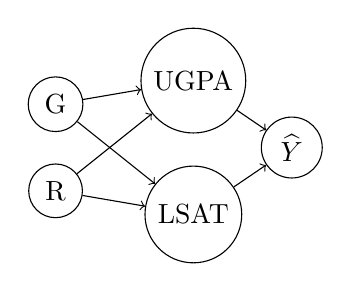
\begin{tikzpicture}
        \node (A1)  at (-1.75, -0.55) [circle, draw]{R};
        \node (A2)  at (-1.75, 0.55) [circle, draw]{G};
        \node (X1) at (0, 0.85) [circle, draw]{UGPA};
        \node (X2) at (0,-0.85) [circle,draw]{LSAT};
        \node (Y)  at (1.25, 0) [circle, draw]{$\widehat{Y}$};
        \draw[->] (A1) to (X1) {};
        \draw[->] (A1) to (X2) {};
        \draw[->] (A2) to (X1) {};
        \draw[->] (A2) to (X2) {};
        \draw[->] (X1) to (Y) {};
        % \draw[->] (X1) to (X2) {};
        \draw[->] (X2) to (Y) {};
    \end{tikzpicture}
\end{figure}
\end{minipage}
\begin{minipage}{.55\linewidth}
\begin{align*}
\mathcal{M} \, & 
\begin{cases}
    R & \leftarrow U_{R}\\
    G & \leftarrow U_G \\
    UGPA & \leftarrow b_U + \beta_1 \cdot R + \lambda_1 \cdot G + U_1, \ \\
    LSAT & \leftarrow  \exp\{b_L + \beta_2 \cdot R + \lambda_2 \cdot G + U_2\}, \\
\end{cases}
\end{align*}
\begin{align*}
    \widehat{Y} & = b(UGPA, LSAT) 
    % \\
    % & = \mathbbm{1}\{(0.6 \cdot UGPA + 0.4 \cdot LSAT) > \psi\}
\end{align*}
\end{minipage}
\caption{The auxiliary causal knowledge for Section~\ref{sec:Experiments.Real}. Let $R$ denote race, $G$ gender, \textit{LSAT} law school admissions test scores, \textit{UGPA} undergraduate grade-point average, and $\hat{Y}$ the admissions decision by $b()$.}
\label{fig:LawSchool}
% \vspace{-2ex}
\end{figure}
%

Let us now consider the law school admissions scenario popularized by \textcite[Figure 2]{Kusner2017CF}.
We use US data from the Law School Admission Council survey \parencite{Wightman1998_LawDataSource}, and recreate an admissions scenario for a top US law school. 
We consider as protected attributes an applicant's gender (\textit{G}, male/female), and race (\textit{R}, white/non-white). 
We add the ADM $b(UGPA, LSAT) = \hat{Y}$, which considers the applicant's undergraduate grade-point average (\textit{UGPA}) and law school admissions test scores (LSAT). 
If an applicant is successful, $\widehat{Y}=1$; otherwise $\widehat{Y}=0$. 
We summarize the scenario in Figure~\ref{fig:LawSchool}.
We define the ADM $b()$ using the median entry requirements for the top US law school to derive the cutoff $\psi$.\footnote{That being Yale University Law School; see \url{https://www.ilrg.com/rankings/law/index/1/asc/Accept}}
Formally, we define $b()$ as $\mathbbm{1}\{(0.6 \cdot UGPA + 0.4 \cdot LSAT) > \psi\}$.
The cutoff is the weighted sum of 60\%  in \textit{UGPA} (3.93 over 4.00), and 40\%  \textit{LSAT} (46.1 over 48), giving a total of 20.8; the maximum possible score given $b()$ is 22. 
The SCM $\mathcal{M}$ and DAG $\mathcal{G}$ follow \textcite{Kusner2017CF},
with $b_U$ and $b_L$ denoting the intercepts; $\beta_1$, $\beta_2$, $\lambda_1$, $\lambda_2$ the weights; and $U_1 \sim \mathcal{N}$ and $U_2 \sim \text{Poi}$ the probability distributions.

We study the behavior of $b()$ toward $G$ and $R$.
The dataset $\mathcal{D}$ contains $n=21790$ applicants, 43.8\% being female, 16.1\% being non-white, and 8.4\% being non-white-female.
%
Despite $b()$ being externally imposed by us for the purpose of illustrating the CST framework, under $b()$ only 0.8\% of the female applicants are successful compared to 1.5\% of the male applicants; similarly, only 0.2\% of the non-white applicants are successful compared to 2.2\% of the white applicants.
It is also the case when considering the intersectional group of non-white-females, with only 0.06\% of these applicants being admitted to law school based on $b()$ compared to the 2.25\% of white-female, non-white-male, and white-male successful applicants.
Notice that $b()$ is highly selective, with an acceptance rate of just 2.31\%, or 505 out of 21790 applicants considered.
Using DP as a fairness metric, $b()$ would still be considered unfair toward female, non-white, and non-white-female applicants.

\subsubsection{Single Discrimination}
\label{sec:Experiments.Real.Single}

%
\begin{table}[t]
\caption{Number (and \% w.r.t.~non-whites) of individual discrimination cases based on $R$ using Figure~\ref{fig:LawSchool}. Marked by * are the statistically significant cases.}
  \label{table:k-results_RACE}
  \centering
  \begin{tabular}{cccccc}
    \toprule
    Method & $k=15$ & $k=30$ & $k=50$ & $k=100$ & $k=250$\\
    \midrule
    CST w/o & 256 (7.3\%) & 309 (8.8\%) & 337 (9.6\%) & 400 (11.4\%)  & 503 (14.4\%) \\
     & 244* (6.9\%) & 301* (8.6\%) & 323* (9.2\%) & 391* (11.2\%)  & 494* (14.1\%) \\
     \midrule
    ST & 33 (0.9 \%) & 51 (1.5\%) & 61 (1.7\%) & 64 (1.8\%) & 78 (2.2\%) \\
    & 28* (0.8\%) & 28* (0.8\%) & 45* (1.3\%) & 47* (1.3\%) & 61 (1.7\%) \\
    \midrule
    CST w/ & 286 (8.2\%) & 309 (8.8\%) & 337 (9.6\%) & 400 (11.4\%)  & 503 (14.4\%)\\
    & 244* (6.9\%) & 301* (8.6\%) & 323* (9.2\%) & 391* (11.2\%)  & 494* (14.1\%) \\
    \midrule
    CF & 231 (6.6\%) & 231 (6.6\%) & 231 (6.6\%) &  231 (6.6\%) &  231 (6.6\%) \\
    & 190* (5.4\%) & 231* (6.6\%) & 231* (6.6\%) & 231* (6.6\%) & 231* (6.6\%) \\
    \bottomrule
  \end{tabular}
\end{table}
%

%
\begin{table}[t]
\caption{Number (and \% w.r.t.~females) of individual discrimination cases based on $G$ Figure~\ref{fig:LawSchool}. Marked by * are the statistically significant cases.}
  \label{table:k-results_GENDER}
  \centering
  \begin{tabular}{cccccc}
    \toprule
    Method & $k=15$ & $k=30$ & $k=50$ & $k=100$ & $k=250$\\
    \midrule
    CST w/o & 78 (0.8\%) & 120 (1.3\%) & 253 (2.7\%) & 296 (3.1\%)  & 493 (5.2\%) \\
     & 43* (0.5\%) & 88* (0.9\%) & 160* (1.7\%) & 221* (2.3\%)  & 341* (3.6\%) \\
     \midrule
    ST & 77 (0.8\%) & 101 (1.1\%) & 229 (2.4\%) & 258 (2.7\%) & 484 (5.1\%) \\
    & 57* (0.6\%) & 69* (0.7\%) & 111* (1.2\%) & 124* (1.3\%) & 366 (3.8\%) \\
    \midrule
    CST w/ & 99 (1.0\%) & 129 (1.4\%) & 267 (2.8\%) & 296 (3.1\%)  & 493 (5.2\%)\\
    & 54* (0.6\%) & 92* (0.9\%) & 160* (1.7\%) & 221* (2.3\%)  & 341* (3.6\%) \\
    \midrule
    CF & 56 (0.6\%) & 56 (0.6\%) & 56 (0.6\%) &  56 (0.6\%) &  56 (0.6\%) \\
    % & 20* (0.2\%) & 15* (0.2\%) & 30* (0.3\%) & 21* (0.2\%) & 32* (0.3\%) \\
    & 20* (0.2\%) & 15* (0.2\%) & 30* (0.3\%) & 21* (0.2\%) & 32* (0.3\%) \\
    \bottomrule
  \end{tabular}
\end{table}
%

Does $b()$ discriminate against non-white applicants? 
To answer this question using CST and CF, we generate the corresponding $\mathcal{D}^{CF}_R$ using Figure~\ref{fig:LawSchool} based in the intervention $do(R:=0)$, or \textit{what would have happened had all law school applicants been white?}
Similarly, does $b()$ discriminate against female applicants?
To answer this question using CST and CF, we generate the corresponding $\mathcal{D}^{CF}_G$ using Figure~\ref{fig:LawSchool} based in the intervention $do(G:=0)$, or \textit{what would have happened had all law school applicants been male?}
Both questions share the same $\mathcal{D}$.
Similar to Section~\ref{sec:Experiments.IllustrativeExample}, we use Definition~\ref{def:IndDisc} for detecting individual discrimination cases and Definition~\ref{def:CIs} for determining whether these cases are statistically significant.
Tables~\ref{table:k-results_RACE} and \ref{table:k-results_GENDER} show the results for all methods.
 
Tables~\ref{table:k-results_RACE} and \ref{table:k-results_GENDER} report similar patterns to those in Table~\ref{table:k-results}.
CST w/o detects a higher number of cases than ST; CST w/ detects a high number of cases than CF; and CST w/ detects a higher number than CST w/o. 
For all these patterns, though, the differences between the corresponding methods is smaller than those observed in Table~\ref{table:k-results}.
This is due to the composition of $\mathcal{D}$ and the nature of $b()$. 
Here, we work with a larger $\mathcal{D}$ (21790 versus 5000 applicants) and a more selective $b()$ (2.31\% versus 53.3\% acceptance rate).
CST w/o and CST w/ in Table~\ref{table:k-results_GENDER} converge already at larger neighborhood sizes, which does not occur in Table~\ref{table:k-results} (there is, though, a clear pattern that it occurs eventually as shown in Figure~\ref{fig:TwoCSTs_k_param}).
We also observe similar patterns once we account for statistical significance with CST w/o and CST w/ reaching the same number of cases in both tables for $k=250$.

%
\begin{figure}[t]
    \begin{subfigure}{.45\linewidth}
    \includegraphics[scale=0.45]{figures/R_all_delta_versus_k.png}
    \caption{}
     % \label{fig:a}
    \end{subfigure}
\hfill
    \begin{subfigure}{.45\linewidth}
    \includegraphics[scale=0.45]{figures/G_all_delta_versus_k.png}
    \caption{}
     % \label{fig:b}
    \end{subfigure}
\medskip
   \begin{subfigure}{.45\linewidth}
    \includegraphics[scale=0.45]{figures/R_all_nums_versus_k.png}
    \caption{}
     % \label{fig:c}
    \end{subfigure}
\hfill
    \begin{subfigure}{.45\linewidth}
    \includegraphics[scale=0.45]{figures/G_all_nums_versus_k.png}
    \caption{}
     % \label{fig:d}
    \end{subfigure}
\caption{Average $\Delta p$ and number of cases for race ($R$) and gender ($G$), respectively. We plot all and statistically significant (sig.) cases for each method.}
\label{fig:LawSchoolSingleDiscrimiantion_allmethods_k_param}
\end{figure}
%

Figure~\ref{fig:LawSchoolSingleDiscrimiantion_allmethods_k_param} supports Tables~\ref{table:k-results_RACE} and \ref{table:k-results_GENDER}, showing the average $\Delta p$ and the number of cases up to $k=500$ for all methods.\footnote{Due the size of $\mathcal{D}$, we run the methods for $k$ equals 1, 15, 30 and between 50-500 in increments of 10.} 
For the average $\Delta p$, as shown in sub-figures (a) and (b), it decreases as $k$ increases, with all methods seemingly converging to a single value.
%
% Notably, 
By observing that, as $k \rightarrow \infty$, the neighborhoods of the complainant and its counterfactual include all protected and unprotected instances, respectively, in $\mathcal{D}$, this value turns out to be the difference in DP: $P(\hat{Y}|A=1) - P(\hat{Y}|A=0)$ (cfr., footnote~\ref{foot:dp}) .
%
The average $\Delta p$ for significant cases is higher to, see ST in (a), or almost the same as, see CST w/ in (a), for all the cases.  
As $k$ increases, the control and tests groups constructed by ST, CST w/o, and CST w/ start considering new instances further away from the search centers and whatever detected initial deviation from $\tau$ dissipates slowly.
%
Similarly, as shown in sub-figures (c) and (d), the number of cases increases as $k$ increases except for CF which is independent of $k$ and its significant cases that are bounded by CF itself. 
We observe the CST versions converging, especially when accounting for statistical significance, while ST remains below both CST versions in (c) and mimics CST w/o in (d).
The number of significant cases is lower to ST in (c), or almost the same as both CST versions in (c) for all cases. 

The number of cases varies across the methods between Tables~\ref{table:k-results_RACE} and \ref{table:k-results_GENDER}. 
This is due to race and gender having different non-protected and protected search spaces.
The results are comparable, but represent separate tests for single discrimination.
Recall that non-whites represent 16.1\% while females represent 43.8\% of $\mathcal{D}$. 
It means that CST has access to a smaller search space when building the control groups for non-white complainants relative to female complainants.
Notably, in Table~\ref{table:k-results_RACE} statistically significant CF cases reach the 231 CF total cases within the $k$ values considered. 
This does not occur in Table~\ref{table:k-results_GENDER} in which the statistically significant CF cases slowly increase, though in a non-monotonically way, toward the 56 CF total cases.
Such oscillation, we believe, is due to the statistical estimator not yet reaching its asymptotic behavior.
These are, though, minor fluctuations as the number of statistically significant cases is around 0.2-0.3\%.\footnote{We use the CI \eqref{eq:CIs} from CST w/ though conditioned on CF discrimination occurring. We only detect 56 cases of CF discrimination (Table~\ref{table:k-results_GENDER}). As $k$ increases, we always look at these complainants.}
In Figure~\ref{fig:LawSchoolSingleDiscrimiantion_allmethods_k_param} we observe this non-monotonic increase for number of cases and decrease for the average $\Delta p$ of cases detected more clearly in the sub-figures (a) and (c) for race than for the sub-figures (b) and (d) for gender. 
The plots for gender are considerably less smooth than those for race. 
The composition of $\mathcal{D}$ clearly plays a role here as females represent 43.8\% and non-whites 16.1\% of the dataset, with the k-NN based methods varying more between iterations as they explore a much denser search space.

\subsubsection{Multidimensional Discrimination}
\label{sec:Experiments.Real.Multi}

We present the results for the forms of multidimensional discrimination, multiple and intersectional.
Given the focus on gender and race, the non-protected group amounts to the non-protected groups based on race and gender: i.e., white and male applicants.
As these two groups of applicants are not mutually exclusive, white-females and non-white-males are also part of the non-protected group.
This point is clearer when we consider the intersection of race and gender and focus on the protected group that is non-white-female applicants: the complementary of such group, meaning the non-protected group, includes white-female, non-white-male, and white-male applicants.

%
\begin{table}[t]
  \caption{Number (and \% w.r.t.~non-white-females) of multiple individual discrimination cases in Section~\ref{sec:Experiments.Real} for $R$ and $G$. Marked by * are the statistically significant cases.}
  \label{table:k-results_Multiple}
  \centering
  \begin{tabular}{cccccc}
    \toprule
    Method & $k=15$ & $k=30$ & $k=50$ & $k=100$ & $k=250$\\
    \midrule
    CST w/o & 8 (0.44\%) & 10 (0.55\%) & 20 (1.09\%) & 20 (1.09\%)  & 40 (2.18\%) \\
     & 4* (0.22\%) & 6* (0.33\%) & 11* (0.60\%) & 17* (0.93\%)  & 24* (1.31\%) \\
     \midrule
    ST & 5 (0.27\%) & 5 (0.27\%) & 12 (0.65\%) & 19 (1.04\%) & 24 (5.1\%) \\
    & 0* (0.0\%) & 0* (0.0\%) & 5* (0.27\%) & 5* (0.27\%)  & 15* (0.82\%) \\
    \midrule
    CST w/ & 9 (0.49\%) & 10 (0.55\%) & 21 (1.15\%) & 20 (1.09\%)  & 40 (2.18\%)\\
    & 4* (0.22\%) & 9* (0.49\%) & 11* (0.60\%) & 17* (0.93\%)  & 24* (1.31\%) \\
    \midrule
    CF & 5 (0.27\%) & 5 (0.27\%) & 5 (0.27\%) & 5 (0.27\%) & 5 (0.27\%) \\
    & 0* (0.0\%) & 3* (0.16\%) & 1* (0.05\%) & 1* (0.05\%) & 2* (0.11\%) \\
    \bottomrule
  \end{tabular}
\end{table}
%

%
\begin{table}[t]
  \caption{Number (and \% w.r.t.~non-white-females) of intersectional individual discrimination cases in Section~\ref{sec:Experiments.Real} for $R \times G$. Marked by * are the statistically significant cases.}
  \label{table:k-results_Intersectional}
  \centering
  \begin{tabular}{cccccc}
    \toprule
    Method & $k=15$ & $k=30$ & $k=50$ & $k=100$ & $k=250$\\
    \midrule
    CST w/o & 130 (7.1\%) & 138 (7.5\%) & 148 (8.1\%) & 160 (8.7\%)  & 199 (10.9\%) \\
    & 130* (7.1\%) & 138* (7.5\%) & 148* (8.1\%) & 160* (8.7\%)  & 199* (10.9\%) \\
     \midrule
    ST & 14 (0.8\%) & 14 (0.8\%) & 17 (0.9\%) & 24 (1.3\%) & 29 (1.6\%) \\
    & 14* (0.8\%) & 14* (0.8\%) & 13* (0.7\%) & 23* (1.3\%)  & 26* (1.4\%) \\
    \midrule
    CST w/ & 130 (7.1\%) & 138 (7.5\%) & 148 (8.1\%) & 160 (8.7\%)  & 199 (10.9\%) \\
    & 130* (7.1\%) & 138* (7.5\%) & 148* (8.1\%) & 160* (8.7\%)  & 199* (10.9\%) \\
    \midrule
    CF & 113 (6.2\%) & 113 (6.2\%) & 113 (6.2\%) & 113 (6.2\%) & 113 (6.2\%) \\
    & 113* (6.2\%) & 113* (6.2\%) & 113* (6.2\%) & 113* (6.2\%) & 113* (6.2\%) \\
    \bottomrule
  \end{tabular}
\end{table}
%

Following Definition~\ref{def:MultipleDisc}, we count as multiple discrimination based on race and gender when $\Delta p > \tau$ occurs separately for each of these protected attributes. 
Only those cases that are statistically significant for each protected attribute under CI \eqref{eq:CIs}---given the Bonferroni corrected $\alpha/2$---amount to statistically significant cases. 
We still rely on the generated $\mathcal{D}_R^{CF}$ and $\mathcal{D}_G^{CF}$ for the construction of the test groups and the original $\mathcal{D}$ for the construction of the control groups.
%
Does $b()$ discriminate against the none-white-female applicants as non-white \textit{and} as female applicants?
We present the results in Table~\ref{table:k-results_Multiple}. 
Figure~\ref{fig:LawSchoolMultiDiscrimination_allmethods_k_param}, as shown in sub-figures (a) and (c), further illustrates the results up to $k=500$. 
For the average $\Delta p$, we average those from cases detected separately under race and gender.

Following Definition~\ref{def:IntersectionaleDisc}, instead, we count intersectional discrimination based on race and gender when $\Delta p > \tau$ occurs for the intersection of these protected attributes. 
In practice, it means constructing the new protected attribute $R \times G$; updating $\mathcal{D}$ into $\mathcal{D}'$, such that $R \times G \in \mathcal{D}'$; and generating $\mathcal{D}'^{CF}$ given Figure~\ref{fig:LawSchool} under $do(R \times G := 0)$.
It implies a single discrimination run but under the ``new'' single attribute $R \times G$, representing the intersection of $R$ and $G$. 
Cases are statistically significant under CI \eqref{eq:CIs} based on $R \times G$.
Formally, in Figure~\ref{fig:LawSchool} we merge the $R$ and $G$ nodes into the single $R \times G$ in $\mathcal{G}$ node and do the same for the corresponding equations in $\mathcal{M}$ by interacting the dummy variables for $R$ and $G$ and re-estimating the regression weights \parencite{Wooldridge2015IntroductoryEconometrics}.
%
Does $b()$ discriminate against the none-white-female applicants?
We present the results in Table~\ref{table:k-results_Intersectional}.
Figure~\ref{fig:LawSchoolMultiDiscrimination_allmethods_k_param}, as shown in sub-figures (b) and (d), further illustrates the results up to $k=500$.

In Tables~\ref{table:k-results_Multiple} and \ref{table:k-results_Intersectional}, the three methods show similar patterns between them.
CST w/o detects more cases relative to ST (including statistically significant cases); CST w/ detects more cases than CF (including statistically significant cases); and the two CST versions converge once statistical significance is considered.
The same line of reasoning used before still applies here for understanding how CST, ST, and CF relate to each other.
The difference is that the protected group and, in turn, the non-protected group are defined by more than one protected attribute.
What is interesting in Table~\ref{table:k-results_Multiple} is that CST w/o and CST w/ converge early on for all cases, not just for those cases that are statistically significant.
We suspect these are cases that are clearly discriminatory under both race and gender, making them likely to be detected by multiple and intersectional discrimination testing.
All cases in Table~\ref{table:k-results_Intersectional} are also statistically significant for all methods.
It is due to $R \times G=1$ representing the most un-favored protected group from the combination of $R$ and $G$, which results in larger $\Delta p$'s and a complete convergence of all and statistically significant cases for all methods relative to multiple discrimination. 
Compare, e.g.,~(a) versus (b) and (c) versus (d) in Figure~\ref{fig:LawSchoolMultiDiscrimination_allmethods_k_param}. 
We discuss the last point in the next section.  

\subsubsection{On Multiple and Intersectional Discrimination}
\label{sec:Experiments.Real.Multiple_vs_Intersectional}

The results from the previous section support claims by legal scholars on the risk of not recognizing intersectional discrimination under non-discrimination law.
These claims, to the best of our knowledge, date back to \textcite{Crenshaw1989_DemarginalizingTheIntersection} and have become prominent again with the ongoing discussion around algorithmic discrimination \parencite{Xenidis2020_TunningEULaw}.
We suspect that, since multiple and intersectional discrimination share the protected group and the non-protected groups, there is a tendency to dismiss the latter as a special case of the former.
An in-depth legal discussion on the tension between multiple and intersectional discrimination is beyond this paper, but Tables~\ref{table:k-results_Multiple} and \ref{table:k-results_Intersectional} support the calls by these researchers to treat intersectional discrimination separate from multiple discrimination.

%
\begin{figure}[t]
    \begin{subfigure}{.45\linewidth}
    \includegraphics[scale=0.45]{figures/Multi_all_deltas_versus_k.png}
    \caption{}
    \end{subfigure}
\hfill
    \begin{subfigure}{.45\linewidth}
    \includegraphics[scale=0.45]{figures/Inter_all_deltas_versus_k.png}
    \caption{}
    \end{subfigure}
    \medskip
    \begin{subfigure}{.45\linewidth}
    \includegraphics[scale=0.45]{figures/Multi_all_nums_versus_k.png}
    \caption{}
     % \label{fig:c}
    \end{subfigure}
\hfill
    \begin{subfigure}{.45\linewidth}
    \includegraphics[scale=0.45]{figures/Inter_all_nums_versus_k.png}
    \caption{}
     % \label{fig:d}
    \end{subfigure}
\caption{Avg. $\Delta p$ and number of cases for multiple (left) and intersectional (right) discrimination on $R$ and $G$. We plot all and statistically significant (sig.) cases for all methods.}
\label{fig:LawSchoolMultiDiscrimination_allmethods_k_param}
\end{figure}
%

We acknowledge that, from a modeling perspective, a difference between Tables~\ref{table:k-results_Multiple} and \ref{table:k-results_Intersectional} is expected since we implement different procedures.
Under multiple discrimination we look at the intersection of two separate single discrimination testing runs, while under intersectional discrimination we look at a single discrimination run representing the intersection. 
%
The claims by legal scholars like \textcite{Crenshaw1989_DemarginalizingTheIntersection, Xenidis2020_TunningEULaw}, however, were not as apparent to us, meaning, in principle, we had no reason to expect a higher number of cases for intersectional discrimination over multiple discrimination.
%
In fact, from a probability theory perspective (read, the conjunction rule), if we had to choose a difference between the Tables~\ref{table:k-results_Multiple} and \ref{table:k-results_Intersectional}, we would have guessed the opposite, with multiple discrimination acting as an upper limit to intersectional discrimination.
Given these results, we now would add that such expectation holds from a modeling perspective if we agree that the intersection of $G$ and $R$ is not its own category. Let us discuss further.

The two modeling procedures allow to represent the case in which $R \times G$ is its own category (intersectional) and in which is just the conjunction of $R$ and $G$ (multiple).
This distinction, with legal origins as already argued \parencite{Crenshaw1989_DemarginalizingTheIntersection}, in fact materializes through the counterfactual representation of each complainant under these two discrimination testing procedures.
Under multiple discrimination, we still rely on $\mathcal{D}_R^{CF}$ and $\mathcal{D}_G^{CF}$ for running the methods separately on $R$ and $G$. 
We look at male and non-white conterfactuals separately. 
Although together they cover all the non-protected groups, they do not do so simultaneously: the complainant under this procedure would have been male or non-white, but not female-non-white.
%
Under intersectional discrimination, instead, we rely on updated factual and counterfactual datasets based on a ``new'' protected attribute $R \times G$. 
The counterfactual for a given compliant implies simultaneously the possibilities of white-male, white-female, and non-white-male, which introduces more randomness.
 
In Figure~\ref{fig:LawSchool}, arguably, the worst-off sub-group between $R$ and $G$ is the group of non-white-female applicants.
% Following the reasoning used in the previous paragraph,
The logic here is that non-white males, meaning $R=1$ and $G=0$, can always resort to their gender and white females, meaning $R=0$ and $G=1$, can always resort to their race.
Instead, non-white females have no single group within the space of $R \times G$ to resort to.
When we test for multiple discrimination we allow for these movements to occur by looking at $R$ and $G$ separately. 
This is because, by not intersecting $R$ and $G$, we do not consider the fact that the group at the intersection never has the choice to resort to a non-protected group. 
This lack of choice is what we represent when we test for intersectional discrimination by looking at $R \times G$ only.
%
The modeling problem for these forms of multidimensional discrimination requires further research with the goal of formalizing the role of the intersection and how it influences the control and test search spaces while taking into account the legal considerations discussed.

Back to Tables~\ref{table:k-results_Multiple} and \ref{table:k-results_Intersectional}, we argue that the observed difference comes from one protected attribute having a stronger influence than the other on the non-protected attributes. 
If that is the case, then testing separately for $R$ and $G$ should show individuals that are discriminated only by one of the protected attributes, which dismisses the multiple discrimination claim.
%
Table~\ref{table:MultivsInter} supports this argument. 
%
Notably, it is for this reason that lawyers discourage multiple discrimination claims and suggest that the complainant focuses on the most dominant protected attribute \parencite{Xenidis2020_TunningEULaw}.

In Table~\ref{table:MultivsInter}, given the results from the previous section, we focus on CST w/o for $k=15$ and look at individual discrimination cases detected as both multiple and intersectional discrimination.
We report the average $p_c$ and $p_t$ for $R$, $G$, and $R \times G$.
% We note that 
All multiple cases are included in the intersectional cases detected by CST w/o.
The first row shows these multiple discrimination cases. We observe that the average $p_c$ is greater than the average $p_t$, and thus the average $\Delta p > \tau$, for $R$, $G$, and $R \times G$. 
These are individual cases that suffer the negative effects of $R$ and $G$, separately and simultaneously, when applying to law school under $b()$.
The second row, instead, shows the intersectional cases only. 
For comparison, we provide the average $p_c$ and $p_t$ for these individuals' single discrimination tests for $R$ and $G$.
We observe that, on average, $R$ is the dominant protected attribute with a considerable difference in the proportion of negative outcomes between the control and test groups. 
This is not the case for $G$ where the average difference is negligible. 
Indeed, for these individuals, by looking at each protected attribute separately, we lose the multiple discrimination case.
In doing so, we also lose focus on what occurs at the intersection of $R \times G$.
The results in Table~\ref{table:MultivsInter} capture this lack of movement between protected and non-protected statuses experienced by those individuals at the bottom of the intersection of $R$ and $G$.

%
\begin{table}[t]
\caption{Avg. $p_c$ and $p_t$ for the ctr's and tst's groups of CST w/o for $k=15$.}
  \label{table:MultivsInter}
  \centering
  \begin{tabular}{ccccccc}
    \toprule
    & \multicolumn{6}{c}{Average}\\
    & $G$'s $p_c$ & $G$'s $p_t$ & $R$'s $p_c$ & $R$'s $p_t$ & $R \times G$'s $p_c$ & $R \times G$'s $p_t$\\
    \midrule
    Multi. and inter. & 0.59 & 0.33 & 0.51 & 0.00 & 0.66 & 0.00 \\
    Inter. only & 0.96 & 0.94 & 0.93 & 0.23 & 0.93 & 0.01 \\
    \bottomrule
  \end{tabular}
\end{table}
%

%
% EOS
%

\section{Results} \label{sec:results}

Figure~\ref{fig:faithfulness_all_main} shows hard faithfulness for multiple tasks and models. 
\textbf{The positional circuits reach high faithfulness at much smaller circuit sizes compared to the non-positional circuits.}

Using LLM-generated schema works well, and adding mask information yields an additional significant boost. Thus, providing the LLM with information about the target models' computation aids in generating effective schemas. 
Discovering circuits with automatic LLM+mask schemas leads to faithulness results that are as good as---and sometimes better than---human-designed schemas. Thus, \textbf{our automated LLM-based schema pipeline discovers circuits with faithfulness comparable to those identified by human experts, even for tasks containing variable-length inputs.}

We now discuss task-specific patterns. In the Greater-Than task, the circuit discovered with the schema via LLM+mask achieves a faithfulness not significantly different from the human-designed schema. The circuit generated solely by the LLM demonstrates lower faithfulness for smaller circuit sizes but achieves higher faithfulness as the circuit size increases. Comparing the  schemas reveals that the schema derived using saliency scores aligns more closely with the human-designed schema. Specifically, both the human-crafted schema and the LLM+mask schema partition the start year to two spans: the first two digits and the last two digits. However, in the LLM-only schema, all four digits are grouped in a single span.

In the IOI task using GPT2-small, we observe that the circuits identified by our automated pipeline closely match the human-designed circuits in faithfulness. However, in the case of Llama-3-8B, the LLM-generated circuits show slightly superior faithfulness compared to human-designed circuits. One plausible explanation is that the IOI task has not been extensively investigated in this larger model, meaning the schema defined for GPT2-small may not optimally capture the nuances of this task in Llama-3-8B. This highlights the importance of tailoring schemas to the specific combination of task and model, rather than extrapolating from results obtained with a different model.

For the Winobias task dataset, similar trends emerge: using the importance mask consistently improves faithfulness scores, making it comparable to the human-defined schema-based circuit.


 

\section{Discussion and Conclusions}
In mechanistic investigations, \textbf{position matters.} Our results suggest it does not make sense in practice to create circuits without considering how distinct the circuit at each position might be.
Theoretical results suggest that it also does not make sense in principle to ignore positionality: \citet{merrill2024expressivepowertransformerschain} show that transformers' expressive power increases with multiple generation steps.
Similarly, accounting for positionality in interpretability methods can enhance their expressive power by capturing the distinct mechanisms processing each token, rather than assuming a single pathway for the entire sequence.

Other interpretability methods such as distributed alignment search (DAS; \citealp{geiger2024das}) already support testing hypotheses about the position of particular causal variables. It would be interesting to directly compare the efficacy of DAS methods when separating results by position versus when aggregating information across positions. Stronger results when separating positional information could help generalize our conclusions to a wider array of causal interpretability methods.



\section*{Limitations}
A key limitation we have discussed is that it is not trivial to handle positional information in tasks where the length of inputs vary. We have proposed an automatic pipeline for generating \emph{and} applying schemas, but future work should explore this further. In particular, because there is no single gold standard for schemas, it is not clear \emph{a priori} what kinds of schemas are generally likely to obtain better trade-offs between faithfulness and circuit size. Devising general principles for effective schema design therefore represents a fruitful avenue for future work. It would also be interesting to observe whether human-generated schemas tend to satisfy these principles, or whether the most effective schemas are not necessarily those that humans are likely to design.

Another key limitation is that a schema requires the same spans to appear in the same order across all examples, such that the edges' direction remains correct across examples. Consequently, two schemas with the same span types but in different orders cannot be evaluated together, as these produce different abstract computation graphs. 

\section*{Acknowledgments}
 This research was supported by the Israel Science
Foundation (grant No.\ 448/20), an Azrieli Foundation
Early Career Faculty Fellowship,  an AI Alignment grant from Open Philanthropy, and a Google gift. HO is supported by the Apple AIML PhD fellowship. DB is supported by a grant from Open Philanthropy. AM is supported by a postdoctoral fellowship under the Zuckerman STEM Leadership Program.
This research was funded by the European Union (ERC, Control-LM, 101165402). Views and opinions expressed are however those of the author(s) only and do not necessarily reflect those of the European Union or the European Research Council Executive Agency. Neither the European Union nor the granting authority can be held responsible for them.



\bibliography{references}

\appendix
% \setcounter{table}{0}
% \renewcommand*{\thetable}{\arabic{table}}
% \renewcommand*{\thefigure}{\arabic{figure}}
\section{Related algorithms and metric caculation}
\label{app:related_algo_metric}

\subsection{Performance-energy Consistency} In this paper, performance-energy consistency refers to the consistency between the results evaluated using an energy model and those evaluated using real-world metrics for the same sample. Specifically, the consistency requires that good samples are assigned low energy, while poor samples are assigned high energy. Performance-energy consistency measures the proportion of element pairs that maintain the same relative order in both permutations \( X \) and \( Y \), where \( X \) and \( Y \) represent the index arrays obtained by sorting the original energy values \( \mathbf{E} = (E_1, E_2, \dots, E_N) \) and performance metric values \( \mathbf{P} = (P_1, P_2, \dots, P_N) \), respectively, in ascending order. In this paper, the energy values are calculated by energy model $E_\theta(x_0)$ for samples $\x_0$. The performance metric values are calculated as the L2 distance between the generated samples $\x_0$ and the ground truth under the given condition.

Let \( X = (X_1, X_2, \dots, X_N) \) and \( Y = (Y_1, Y_2, \dots, Y_N) \) be the index arrays obtained by sorting the original energy values \( \mathbf{E} = (E_1, E_2, \dots, E_N) \) and performance metric values \( \mathbf{P} = (P_1, P_2, \dots, P_N) \), respectively, in ascending order. Specifically, \( X_i \) is the rank of the \( i \)-th sample in the sorted energy values \( \mathbf{E} \), and \( Y_i \) is the rank of the \( i \)-th sample in the sorted performance metric values \( \mathbf{P} \).

\textbf{Consistency Definition:}
The \textbf{consistency} is defined as the proportion of consistent pairs \( (i, j) \) where \( i < j \) and the relative order of \( i \) and \( j \) in \( X \) is the same as in \( Y \). Specifically:
\[
\text{Consistency} = \frac{1}{\binom{N}{2}} \sum_{i=1}^{N-1} \sum_{j=i+1}^{N} \mathbb{I}\left( (X_i < X_j \land Y_i < Y_j) \lor (X_i > X_j \land Y_i > Y_j) \right),
\]
where:
\begin{itemize}
    \item \( \binom{N}{2} = \frac{N(N-1)}{2} \) is the total number of pairs \( (i, j) \) with \( i < j \),
    \item \( \mathbb{I}[\cdot] \) is the indicator function, which evaluates to 1 if the condition inside the brackets holds (i.e., the relative order is consistent), and 0 otherwise.
\end{itemize}
\subsection{Adversarial sampling}
During the sampling process, energy optimization often gets trapped in local minima or incorrect global minima, making it difficult to escape and hindering the sampling of high-quality samples.
\subsection{Negative Sample Generation} Negative samples are generated by introducing noise into the positive sample \( x_0 \). In the Maze and Sudoku experiments, permutation noise is applied to the channel dimension to induce significant changes in the solution. Other noise types can be used, as this remains a hyperparameter choice. Specifically, we first randomly sample two scalars \( p_1 \) and \( p_2 \) from a uniform distribution in the interval \( [0, 1] \), i.e., \( p_1, p_2 \sim \text{Uniform}(0, 1) \) ($p_1<p_2$). Then, for each channel position of the positive sample \( x_0 \), we swap the channel positions with probabilities \( p_1 \) and \( p_2 \), resulting in \( x_0^{-} \) and \( x_0^{--} \), such that the L2 distance between \( x_0^{-} \) and \( x_0 \) is smaller than the L2 distance between \( x_0^{--} \) and \( x_0 \). For other noise types, such as Gaussian noise, we normalize the L2 norm of the noise and apply noise at different scales to ensure that the L2 distance from \( x_0^{-} \) to \( x_0 \) is smaller than the L2 distance from \( x_0^{--} \) to \( x_0 \).


\subsection{Linear-regression algorithm} Given three points \((x_1, y_1)\), \((x_2, y_2)\), and \((x_3, y_3)\), we wish to fit a line of the form ~\cite{lane2003introduction}:

\[
y = kx + b
\]
The mean of the \(x\)-coordinates and the mean of the \(y\)-coordinates are:
\[
\bar{x} = \frac{1}{3}(x_1 + x_2 + x_3), \quad \bar{y} = \frac{1}{3}(y_1 + y_2 + y_3)
\]
The slope \(k\) of the best-fit line is given by the formula:

\[
k = \frac{\sum_{i=1}^{3} (x_i - \bar{x})(y_i - \bar{y})}{\sum_{i=1}^{3} (x_i - \bar{x})^2}
\]
This formula represents the least-squares solution for the slope.
Once the slope \(k\) is determined, the intercept \(b\) can be calculated as:
\[
b = \bar{y} - k\bar{x}
\]
The equation of the best-fit line is:
\[
\hat{y} = kx + b
\]
\section{Details of experiments}
\label{app:Exp_detail}
\subsection{Detais of Sudoku experiments}
\label{app:Exp_sudoku}
For Sudoku experiment, the dataset, model architecture, and training configurations are adopted from \citet{du2024learning}. We mainly use solving success rate to evaluate different models. Model backbone and training configurations can be found in Fig. \ref{fig:sudoku_ebm} and Table \ref{tab:sudoku_exp_detail}, respectively. All the exploration hyperparameters $c$ are set as 100 for Sudoku task.
\begin{figure}[H]
\begin{minipage}{0.9\textwidth}
\centering
\small
\begin{tabular}{c}
    \toprule
    3x3 Conv2D, 384 \\
    \midrule
    Resblock 384 \\
    \midrule
    Resblock 384 \\
    \midrule
    Resblock 384 \\
    \midrule
    Resblock 384 \\
    \midrule
    Resblock 384 \\
    \midrule
    Resblock 384 \\
    \midrule
    3x3 Conv2D, 9 \\ 
    \bottomrule
\end{tabular}
\caption{The model architecture for \proj on Sudoku task. The energy value is computed using the L2 norm of the final predicted output similar to \citet{du2023reduce}, while the output is directly used as noise prediction for the diffusion baseline.}
\label{fig:sudoku_ebm}
\end{minipage}
\end{figure}
\begin{table}[ht]
  \begin{center}
    \caption{\textbf{Details of  training for Sudoku task}. }
    \vskip -0.15in
    \label{tab:2d_model_architecture}
    \begin{tabular}{l|c} % <-- Alignments: 1st column left, 2nd middle and 3rd right, with vertical lines in between
    \multicolumn{2}{l}{}\\
      \hline
       \multicolumn{1}{l|}{Training configurations } & \multicolumn{1}{l}{}\\
      \hline
      Number of training steps & 100000  \\
      Training batch size & 64 \\
      Learning rate & 0.0001 \\
      Diffusion steps & 10 \\
      Inner loop optimization steps & 20 \\
      Denoising loss type & MSE \\
      Optimizer & Adam \\
        \hline
    \end{tabular}
      \label{tab:sudoku_exp_detail}
  \end{center}
\end{table}
\subsection{Details of Maze experiments}
\label{app:Exp_maze}
The details of maze experiments and model backbone are provided in Table \ref{tab:maze_exp_detail} and Fig. \ref{fig:maze_ebm}, respectively. The key metric, the maze-solving success rate is defined as the proportion of model-generated paths that have no breakpoints, do not overlap with walls, and begin and end at the start and target points, respectively. Maze datasets are generated by \citet{ivanitskiy2023configurable}, and detailed hyperparameter configurations are in Table \ref{tab:maze_exp_detail}. All the exploration hyperparameters $c$ are set as 100 for Maze task.
\begin{figure}[H]
\begin{minipage}{0.9\textwidth}
\centering
\small
\begin{tabular}{c}
    \toprule
    3x3 Conv2D, 384 \\
    \midrule
    Resblock 384 \\
    \midrule
    Resblock 384 \\
    \midrule
    Resblock 384 \\
    \midrule
    Resblock 384 \\
    \midrule
    Resblock 384 \\
    \midrule
    Resblock 384 \\
    \midrule
    3x3 Conv2D, 9 \\ 
    \bottomrule
\end{tabular}
\caption{The model architecture for \proj on Maze task. The energy value is computed using the L2 norm of the final predicted output similar to \citet{du2023reduce}, while the output is directly used as noise prediction for the diffusion baseline.}
\label{fig:maze_ebm}
\end{minipage}
\end{figure}
\begin{table}[ht]
  \begin{center}
    \caption{\textbf{Details of Maze dataset, training}. }
    \vskip -0.15in
    \label{tab:2d_model_architecture}
    \begin{tabular}{l|c} % <-- Alignments: 1st column left, 2nd middle and 3rd right, with vertical lines in between
    \multicolumn{2}{l}{}\\
      \hline
      \multicolumn{1}{l|}{Dataset:} & \multicolumn{1}{l}{}\\ 
      \hline
      Size of training dataset with grid size 4 & 10219   \\
      Size of training dataset with grid size 5 & 9394   \\
      Size of training dataset with grid size 6 & 10295  \\
      Minimum length of solution path & 5 \\
      Algorithm to generate the maze & DFS \\
      Size of test dataset with grid size 6 & 837   \\
      Size of test dataset with grid size 8 & 888   \\
      Size of test dataset with grid size 10 & 948   \\
      Size of test dataset with grid size 12 & 960   \\
      Size of test dataset with grid size 15 & 975   \\
      Size of test dataset with grid size 20 & 978   \\
      Size of test dataset with grid size 30 & 994   \\
      \hline
       \multicolumn{1}{l|}{Training configurations } & \multicolumn{1}{l}{}\\
      \hline
      Number of training steps & 200000  \\
      Training batch size & 64 \\
      Learning rate & 0.0001 \\
      Diffusion steps & 10 \\
      Inner loop optimization steps & 20 \\
      Denoising loss type & MSE + MAE \\
      Optimizer & Adam \\
        \hline
    \end{tabular}
      \label{tab:maze_exp_detail}
  \end{center}
\end{table}

\section{Performance sensitivity to hyperparameters}
\label{app:hyperparameters_sensitivity}

% inner loop opt steps, mcts noise scale(original model, mixed trained model hMCTS & Random search) more visualizations?
In this subsection, we analyze the impact of several hyperparameters on the experimental results. As shown in Table \ref{tab:maze_noise_scale}, the influence of different noise scales on the performance of various methods is presented. The hMCTS denoising and random search require a relatively larger noise scale to better expand the search space and improve final performance, while the diffusion model with naive inference performs best with a smaller noise scale. As demonstrated in Table \ref{tab:maze_inner_loop_opt} and Fig. \ref{fig:maze_opt_step}, the effect of varying inner-loop optimization steps on the results is also analyzed. It can be observed that performance improves gradually with an increasing number of steps, and after 5 steps, the performance stabilizes and the improvement slows down. Therefore, we chose 5 inner-loop optimization steps for the Maze experiments in this paper.
\begin{figure}[h!]
\vskip 0.2in
\begin{center}
\centerline{\includegraphics[width=0.55\textwidth]{fig/maze_optimization_steps_vs_values.pdf}}
\caption{Visualization of success rate across different number of inner-loop optimization steps on Maze with grid size $\mathbf{15\times15}$. }
\label{fig:maze_opt_step}
\end{center}
\vskip -0.2in
\end{figure}
\begin{table}[ht]
\caption{Success rate across the different number of inner-loop optimization step on Maze with grid size \textbf{15}. }
\label{tab:maze_inner_loop_opt}
\vskip 0.15in
\begin{center}
\resizebox{0.85\textwidth}{!}{ % Resize the table to fit within a single column
\begin{tabular}{l|cccccccccc}
\toprule
 &\multicolumn{10}{c}{\textbf{Number of optimization step}} \\
\cmidrule(lr){2-11} 
\textbf{Methods}                & 1               & 2               & 3               & 4               & 5               & 6               & 7               & 8               & 9 &10        \\
\midrule
T-SCEND tr. (ours), Naive inference & 0.0000 & 0.1562 & 0.2109 & 0.2734 & 0.2812 & 0.2734 & 0.2812 & 0.2969 & 0.2969 & 0.2969\\
\bottomrule
\end{tabular}
}
\end{center}
\vskip -0.1in
\end{table}
\begin{table}[ht]
\caption{Success rate across different noise scales on Maze with grid size \textbf{15}. }
\label{tab:maze_noise_scale}
\vskip 0.15in
\begin{center}
\resizebox{1\textwidth}{!}{ % Resize the table to fit within a single column
\begin{tabular}{l|cccccccccc}
\toprule
 &\multicolumn{10}{c}{\textbf{Noise scale}} \\
\cmidrule(lr){2-11} 
\textbf{Methods}                & 0.1               & 0.2               & 0.3               & 0.4               & 0.5               & 0.6               & 0.7               & 0.8               & 0.9 &1.0        \\
\midrule
T-SCEND tr. (ours), hMCTS denoising (energy)               & 0.3828 & 0.4375 & 0.5312 & 0.6094 & 0.6562 & 0.6953 & 0.7031 & 0.7344 & 0.7734 & 0.7969 \\
T-SCEND tr. (ours), naive inference                    & 0.3125 & 0.2656 & 0.2578 & 0.2344 & 0.2422 & 0.2656 & 0.2578 & 0.2422 & 0.2500 & 0.2500 \\
T-SCEND tr. (ours), Random search(energy)      & 0.3906 & 0.4453 & 0.5312 & 0.5703 & 0.5938 & 0.6328 & 0.6641 & 0.6719 & 0.6797 & 0.6562 \\
\bottomrule
\end{tabular}
}
\end{center}
\vskip -0.1in
\end{table}
\section{Additional results}
\label{app:additional_results}
\begin{figure}[h!]
\vskip 0.2in
\begin{center}
\centerline{\includegraphics[width=0.6\textwidth]{fig/maze_success_rate_vs_ts.pdf}}
\caption{Visualization of Success rate across different MCTS start step $t_s$. }
\label{fig:maze_success_rate_vs_ts}
\end{center}
\vskip -0.2in
\end{figure}
The parameter \( t_s \) controls the proportion of the total inference budget allocated to MCTS denoising. When \( t_s = 9 \), it means only MCTS denoising is used, while \( t_s = 0 \) means only best-of-N random search is employed. For \( 0 < t_s < 9 \), hMCTS denoising is applied. As shown in Table \ref{tab:maze_mcts_start_step} and Fig. \ref{fig:maze_success_rate_vs_ts}, there is a noticeable peak in model performance as \( t_s \) varies.
\begin{table}[h!]
\caption{Success rate of hMCTS denoising on Maze with grid size \textbf{15} across different MCTS start steps. }
\label{tab:maze_mcts_start_step}
\vskip 0.15in
\begin{center}
\resizebox{\textwidth}{!}{ % Resize the table to fit within a single column
\begin{tabular}{l|cccccccccc}
\toprule
\cmidrule(lr){2-11} 
\textbf{Methods} & 0               & 1               & 2               & 3               & 4               & 5               & 6               & 7               & 8               & 9         \\
\midrule
Original, hMCTS denoising (energy)      & 0.0781 & 0.0703 & 0.0859& 0.0781 & 0.1250& 0.1484& 0.1250 & 0.0781 & 0.0625 & 0.0703\\
T-SCEND tr. (ours), hMCTS denoising (energy)   & 0.6562 & 0.6094& 0.6641 & 0.7969 & 0.7969 & 0.6406& 0.4922 & 0.4922 & 0.4609 & 0.4453 \\
\bottomrule
\end{tabular}
}
\end{center}
\vskip -0.1in
\end{table}

\begin{table}[h!]
\caption{Success rate of Random search for different training methods on Maze with grid size \textbf{15} and Sudoku harder dataset guided with ground truth accuracy. Untrained, Random search (gt) represents use ground truth to guide the random search.  Here, $L=N$. Bold font denotes the best model. }
\label{tab:maze_diffus_baseline_diversity}
\vskip 0.15in
\begin{center}
\resizebox{\textwidth}{!}{ % Resize the table to fit within a single column
\begin{tabular}{l|cccccc|ccccccc}
\toprule
\multicolumn{1}{c|}{} & \multicolumn{6}{c}{\textbf{Maze success rate}} & \multicolumn{7}{c}{\textbf{Sudoku success rate}}\\ 
\cmidrule(lr){2-14} 
\textbf{Methods} & \textbf{$N$=1} & \textbf{$N$=11} & \textbf{$N$=21} & \textbf{$N$=41} & \textbf{$N$=81} & \textbf{$N$=161} &\textbf{$N$=1} & \textbf{$N$=11} & \textbf{$N$=21} & \textbf{$N$=41} & \textbf{$N$=81} & \textbf{$N$=161} & \textbf{$N$=321} \\
\midrule
Untrained, Random search (gt) & 0.0000 & 0.0000 & 0.0000 & 0.0000 & 0.0000 & 0.0000 & 0.0000 & 0.0000 & 0.0000 & 0.0000 & 0.0000 & 0.0000 & 0.0000 \\ 
Original, Random search (gt) & 0.0625 & 0.1250 & 0.1094 & 0.1328 & 0.1719 & 0.1719 & 0.0859 & 0.1641 & 0.2188 & 0.2344 & 0.2422 & 0.2656 & 0.2969 \\
DDPM, Random search (gt) & 0.0312&0.1094&0.1587&0.1746&0.2031&0.2422& 0.0000          & 0.0000          & 0.0000          & 0.0000          & 0.0000          & 0.0000          & 0.0156 \\
T-SCEND tr. w/o LRNCL, Random search (gt) & \textbf{0.2500} & \textbf{0.5078} & \textbf{0.5938} & \textbf{0.6562} & \textbf{0.7109} & \textbf{0.7422} & \textbf{0.1094} & \textbf{0.2578} & \textbf{0.2969} & \textbf{0.3438} & \textbf{0.3750} & \textbf{0.3828} & \textbf{0.4219} \\ 
\bottomrule
\end{tabular}
}
\end{center}
\vskip -0.1in
\end{table}
\begin{table}[h!]
\caption{Success rate and element-wise accuracy of Random search for different training methods on Sudoku harder dataset guided with ground truth accuracy. Here, $L=N$. Bold font denotes the best model. }
\label{tab:sudoku_diffus_baseline_ddpm}
\vskip 0.15in
\begin{center}
\resizebox{1\textwidth}{!}{ % Resize the table to fit within a single column
\begin{tabular}{l|ccccccc|ccccccc}
\toprule
& \multicolumn{7}{c|}{\textbf{Success rate}} & \multicolumn{7}{c}{\textbf{Element-wise} accuracy}\\
\cmidrule(lr){2-15} 
Methods &\textbf{$N$=1} & \textbf{$N$=11} & \textbf{$N$=21} & \textbf{$N$=41} & \textbf{$N$=81} & \textbf{$N$=161} & \textbf{$N$=321} &
\textbf{$N$=1} & \textbf{$N$=11} & \textbf{$N$=21} & \textbf{$N$=41} & \textbf{$N$=81} & \textbf{$N$=161} & \textbf{$N$=321} \\
\midrule
DDPM, Random search, GT accuracy guided     & 0.0000          & 0.0000          & 0.0000          & 0.0000          & 0.0000          & 0.0000          & 0.0156          & 0.5071          & 0.6089          & 0.6316          & 0.6492          & 0.6691          & 0.6881          & 0.6999          \\
Original, Random search, GT accuracy guided & 0.0781          & 0.1641          & 0.2188          & 0.2344          & 0.2422          & 0.2656          & 0.2812          & \textbf{0.6650} & 0.7731          & 0.7952          & 0.8036          & 0.8217          & 0.8347          & 0.8491          \\
T-SCEND tr. w/o LRNCL, Random search, GT accuracy guided            & \textbf{0.1094} & \textbf{0.2578} & \textbf{0.2969} & \textbf{0.3438} & \textbf{0.3750} & \textbf{0.3828} & \textbf{0.4219} & 0.6442 & \textbf{0.7855} & \textbf{0.8096} & \textbf{0.8317} & \textbf{0.8466} & \textbf{0.8628} & \textbf{0.8854} \\ 
\bottomrule
\end{tabular}
}
\end{center}
\vskip -0.1in
\end{table}





% \begin{table}[]
% \caption{Success rate of mixed inference on Maze with grid size \textbf{15} across different MCTS start steps. Bold font denotes the best model.}
% \label{tab:maze_mcts_start_step}
% \begin{tabular}{lllllllllll}
% \cline{1-1}
% \multicolumn{1}{|l|}{Method} & \multicolumn{10}{c}{MCTS start step}                                                                                                                                              \\
% \multicolumn{1}{|l|}{}                        & 0               & 1               & 2               & 3               & 4               & 5               & 6               & 7               & 8               & 9               \\ \cline{1-1}
% Mixed inference, KL \& LRNCL ,Energy guided   & 0.6562 ± 0.4750 & 0.6094 ± 0.4879 & 0.6641 ± 0.4723 & 0.7969 ± 0.4023 & 0.7969 ± 0.4023 & 0.6406 ± 0.4798 & 0.4922 ± 0.4999 & 0.4922 ± 0.4999 & 0.4609 ± 0.4985 & 0.4453 ± 0.4970 \\
% Mixed inference, Original, Energy guided      & 0.0781 ± 0.2684 & 0.0703 ± 0.2557 & 0.0859 ± 0.2803 & 0.0781 ± 0.2684 & 0.1250 ± 0.3307 & 0.1484 ± 0.3555 & 0.1250 ± 0.3307 & 0.0781 ± 0.2684 & 0.0625 ± 0.2421 & 0.0703 ± 0.2557
% \end{tabular}
% \end{table}
\section{Limitations and future work}
\label{app:limit_future} 
Our inference framework primarily relies on MCTS, which presents two key limitations: (1) limited compatibility with parallel computing, and (2) challenges in effectively evaluating node quality during the early stages of denoising. Future work could explore integrating alternative search strategies, such as those proposed by \citet{wu2024inference}. Additionally, to enhance performance-energy consistency, we introduce linear-regression negative contrastive learning, which enforces a linear relationship between energy and the distance to real samples. Further investigation is needed to assess the broader implications of this constraint and explore alternative regularization approaches. Lastly, while our current implementation utilizes Gaussian noise for branching, other diffusion-based branching mechanisms remain an open area for exploration.
\section{Visualization of results}
\label{app:vis_results}
\subsection{Visualization of Maze experiments}
\label{app:maze_vis}
This section presents visualizations of the training in Fig. \ref{fig:maze_training_vis}, test Maze data in Fig. \ref{fig:maze_test_vis}, and samples generated by different methods in Fig. \ref{fig:maze_samples_diff}. In the visuals, black pixels denote walls, green represents the starting point, red represents the goal point, blue marks the solved path, and white represents the feasible area. All visualizations are based on a few representative samples. The results from the training and test sets clearly show that the tasks in the test set are notably more challenging than those in the training set. Visual comparisons of samples generated by different methods reveal that the originally trained model, regardless of the inference strategy, performs consistently worse than \proj.
\begin{figure}[tb]
\vskip 0.2in
\begin{center}
\centerline{\includegraphics[width=0.8\textwidth]{fig/maze_plot_multi_grid_size_appendix_train.pdf}}
\caption{Visualization of training maze dataset. }
\label{fig:maze_training_vis}
\end{center}
\vskip -0.2in
\end{figure}

\begin{figure}[ht]
\vskip 0.2in
\begin{center}
\centerline{\includegraphics[width=0.8\textwidth]{fig/maze_plot_multi_grid_size_appendix_test.pdf}}
\caption{Visualization of test maze dataset, where the blue paths are ground-truth solutions.}
\label{fig:maze_test_vis}
\end{center}
\vskip -0.2in
\end{figure}

\begin{figure}[ht]
\vskip 0.2in
\begin{center}
\centerline{\includegraphics[width=0.8\textwidth]{fig/maze_plot_diff.pdf}}
\caption{Visualization of samples generated by different training and inference methods.}
\label{fig:maze_samples_diff}
\end{center}
\vskip -0.2in
\end{figure}
\subsection{Visualization of Sudoku experiments}
\label{app:sudoku_vis}

\begin{figure}[ht]
% \vskip 0.2in
\begin{center}
\centerline{\includegraphics[width=0.7\textwidth]{fig/sudoku_train_test_samples.pdf}}
\caption{Visualization of training and test Sudoku dataset.}
\label{fig:sudoku_training_test_vis}
\end{center}
% \vskip -0.2in
\end{figure}

\begin{figure}[ht]

\vskip 0.2in
\begin{center}
\centerline{\includegraphics[width=0.7\textwidth]{fig/sudoku_plot_diff.pdf}}
\caption{Visualization of samples generated by different training and inference methods.}
\label{fig:sudoku_samples_diff}
\end{center}
\vskip -0.2in
\end{figure}

This section presents visualizations of the training and test Sudoku data in Fig.~\ref{fig:sudoku_training_test_vis}, and representative samples generated by different methods in Fig.~\ref{fig:sudoku_samples_diff}. In the
visuals, black numbers denote the condition, green numbers represent correct predictions, and red numbers represent wrong predictions. All visualizations are derived from a few representative samples. The comparison between the training and test sets clearly indicates that the tasks in the test set are significantly more difficult than those in the training set. When comparing the samples generated by different methods, it is evident that the originally trained model, regardless of the inference strategy, consistently underperforms compared to \proj.

% training dataset, landscape visualization, solution of different models
% \section{Analysis of failure case}
% \tao{TODO}
% \jiashu{TODO}
% \label{app:failure_analysis} 
% training dataset, test dataset, solutions of different models


\end{document}

